% Szglab4
% ===========================================================================

\input{includes/header}
\usepackage{color}
\usepackage{ifthen}
\usepackage{ifpdf}
\ifpdf% 
  \usepackage[pdftex]{graphicx}
  \pdfcompresslevel=9
  \DeclareGraphicsRule{*}{mps}{*}{}
\else
  \usepackage[dvips]{graphicx}
\fi

\newcommand{\entityintro}[3]{%
  \hbox to \hsize{%
    \vbox{%
      \hbox to .2in{}%
    }%
    {\bf  #1}%
    \dotfill\pageref{#2}%
  }
  \makebox[\hsize]{%
    \parbox{.4in}{}%
    \parbox[l]{5in}{%
      \vspace{1mm}%
      #3%
      \vspace{1mm}%
    }%
  }%
}
\newcommand{\refdefined}[1]{
\expandafter\ifx\csname r@#1\endcsname\relax
\relax\else
{$($in \ref{#1}, page \pageref{#1}$)$}\fi}
\date{null}
\chardef\textbackslash=`\\


\csapat{finalize}{23}
  \konzulens{Hartung István}
  \taga{Szőke}{C1GM9G}{istvan.szoken@gmail.com}
  \tagb{Paral}{C0ONDZ}{paralzsolt@gmail.com}
  \tagc{Nyári}{QXW779}{nyaridavid@gmail.com}
  \tagd{Nagy}{ISVSOU}{gergo.nagy094@gmail.com}

\datum{\today}


\begin{document}

%\fedlap{2. Követelmény, projekt, funkcionalitás}
%\fedlap{3. Analízis modell kidolgozása 1}
%\fedlap{4. Analízis modell kidolgozása 2}
\fedlap{5. Szkeleton tervezése}
%\fedlap{6. Szkeleton beadása}
%\fedlap{7. Prototípus koncepciója}
%\fedlap{8. Részletes tervek}
%\fedlap{9. Prototípus készítése, tesztelése}
%\fedlap{10. Prototípus beadása}
%\fedlap{11. Grafikus felület specifikálása}
%\fedlap{12. Grafikus változat készítése}
%\fedlap{13. Grafikus változat beadása}
%\fedlap{14. Összefoglalás}

% Table of Contents and Figures
\clearpage \tableofcontents \pagestyle{fancy}
\clearpage \listoffigures \pagestyle{fancy}

%\setcounter{chapter}{1}
%% Szglab4
% ===========================================================================

\chapter{Követelmény, projekt, funkcionalitás}

\thispagestyle{fancy}

\section{Bevezetés}

\subsection{Cél}
\comment{A dokumentum célja.}

\subsection{Szakterület}
A projekt célja egy egyszerű számítógépes játék létrehozása a RUP fejlesztési módszer segítségével. A szoftvernek teljesítenie kell a Szoftver laboratórium IV. tárgy által adott specifikációban megfogalmazott követelményeket. \\ 
Az elkészült szoftver egy játékprogram, így nem egy hagyományos értelemben vett szakterület számára készül, hanem általános szórakoztatás céljából.

\subsection{Definíciók, rövidítések}
\comment{A dokumentumban használt definíciók, rövidítések magyarázata.}

\subsection{Hivatkozások}
\comment{A dokumentumban használt anyagok, web-oldalak felsorolása}

\subsection{Összefoglalás}
\comment{A dokumentum további részeinek rövid ismertetése}

\section{Áttekintés}

\subsection{Általános áttekintés}
%\comment{A kialakítandó szoftver legmagasabb szintű architekturális képe. A fontosabb alrendszerek felsorolása, a közöttük kialakítandó interfészek lényege, a felhasználói kapcsolatok alapja. Esetleges hálózati és adattárolási elvárások.}

\indent A kialakítandó szoftver alapvetően egy játékprogram \emph{(továbbiakban: játék)}. Több rendszerre és alrendszerre is szükségünk van ahhoz, hogy a felhasználóval \emph{(továbbiakban: játékos)} a kapcsolatot tartsuk és számára a megfelelő játékélményt prezentáljuk.\\
\indent Három alapvető működési egységgel rendelkezik majd a program. Ezek pedig a következő funkciókat ellátó alrendszerek:
\begin{enumerate}
	\setlength\itemsep{0pt}
	\item A játékostól a játék irányába vett interakció
	\item A játéktól a játékos felé történő visszajelzés 
	\item A játék logikájának és állapotának kezelése
\end{enumerate}
Ezen rendszerek között kialakítandó interfészeket úgy kell megvalósítani, hogy azok biztosítsák a játékos számára az alkalmazásnak a gördülékeny működését. Ebből a felhasználónak prezentált kezelőfelületekkel az első két alrendszer rendelkezik.\\
\indent A programnak feltétlen szüksége lesz adattárolási lehetőségre, hogy a a játékos kérésére a játék állását el lehessen tárolni, és azt későbbi továbbjátszás céljából vissza állítható legyen.

\subsection{Funkciók}
\comment{A feladat kb. 4000 karakteres (kb 1,5 oldal) részletezettségű magyar nyelvű leírása. Nem szerepelhetnek informatikai kifejezések.}

\subsection{Felhasználók}
\comment{A felhasználók jellemzői, tulajdonságai}


\subsection{Korlátozások}
\comment{Az elkészítendő szoftverre vonatkozó – általában nem funkcionális - előírások, korlátozások.}

\subsection{Feltételezések, kapcsolatok}
\comment{A dokumentumban használt anyagok, web-oldalak felsorolása}

\section{Követelmények}
\subsection{Funkcionális követelmények}
\comment{Az alábbi táblázat kitöltésével készítendő. Dolgozzon ki követelmény azonosító rendszert! Az ellenőrzés módja szokásosan bemutatás és/vagy kiértékelés. Prioritás lehet alapvető, fontos, opcionális. Az alapvető követelmények nem teljesítése végzetes. Forrás alatt a követelményt előíró anyagot, szervezetet kell érteni. Esetünkben forrás lehet maga a csapat is, mikor ő talál ki követelményt. Use-case-ek alatt az adott követelményt megvalósító használati esete(ke)t kell megadni.}

% Azonosító, Leírás, Ellenőrzés, Prioritás, Forrás, Use-case, Komment
\begin{longtable}{| l | l | l | l | l | l | l |}
\hline
\textbf{Azonosító}   & \textbf{Leírás} & \textbf{Ellenőrzés} & \textbf{Prioritás} & \textbf{Forrás} & \textbf{Use-case} & \textbf{Komment} \tabularnewline
\hline\hline
... & ... & ... & ... & ... & ... & ... \tabularnewline
\hline
\end{longtable}

\subsection{Erőforrásokkal kapcsolatos követelmények}

% Azonosító, Leírás, Ellenőrzés, Prioritás, Forrás, Komment
\begin{tabularx}{\linewidth}{| l | X | l | l | l | X |}
\hline
\textbf{Azonosító}   & \textbf{Leírás} & \textbf{Ellenőrzés} & \textbf{Prioritás} & \textbf{Forrás} & \textbf{Komment} \tabularnewline
\hline\hline
\endhead
E001 & JRE 6 vagy újabb & bemutatás & alapvető & megrendelő &  \tabularnewline \hline
E002 & JRE-hez szükséges minimális rendszerkövetelményekkel rendelkező számítógép & bemutatás & alapvető & megrendelő & \tabularnewline \hline
E003 & Alapvető perifériák & bemutatás & alapvető & megrendelő & monitor, egér, billentyűzet \tabularnewline \hline
E004 & Git & nincs & alapvető & csapat & verziókezelő \tabularnewline \hline
E005 & GitHub & nincs & alapvető & csapat & account minden csapattag részére  \tabularnewline \hline
E006 & TravisCI & nincs & alapvető & csapat & continous integration \tabularnewline \hline
E007 & Coverity & nincs & alapvető & csapat & statikus ellenörző \tabularnewline \hline
E008 & Waffle.io & nincs & opcionális & csapat & projekt management \tabularnewline \hline
E009 & JDK 6 vagy újabb & nincs & alapvető & csapat & \tabularnewline \hline
E010 & Gradle & nincs & alapvető & csapat & build rendszer  \tabularnewline \hline
E011 & Vim & nincs & opcionális & csapat & szövegszerkesztő \tabularnewline \hline 
E012 & GEdit & nincs & opcionális & csapat & szövegszerkesztő \tabularnewline \hline
E013 & Eclipse & nincs & opcionális & csapat & IDE \tabularnewline \hline
E014 & IntelliJ IDEA & nincs & opcionális & csapat & IDE \tabularnewline \hline
E015 & LaTeX & nincs & alapvető & csapat & dokumentáció készítéséhez \tabularnewline \hline
E016 & TeXStudio & nincs & opcionális & csapat & LaTeX IDE \tabularnewline \hline
E017 & Visual Paradigm & nincs & alapvető & csapat & UML IDE \tabularnewline
\hline
\end{tabularx}

\subsection{Átadással kapcsolatos követelmények}

% Azonosító, Leírás, Ellenőrzés, Prioritás, Forrás, Komment
\begin{tabularx}{\linewidth}{| l | X | l | l | l | X |}
\hline
\textbf{Azonosító}   & \textbf{Leírás} & \textbf{Ellenőrzés} & \textbf{Prioritás} & \textbf{Forrás} & \textbf{Komment} \tabularnewline
\hline\hline
\endhead
A001 & Dokumentáció beadás & bemutatás & alapvető & megrendelő & heti rendszerességel, hétfőnként \tabularnewline \hline
A002 & Szkeleton beadás & beadás & alapvető & megrendelő & márc. 23., beadórendszerben \tabularnewline \hline
A003 & Szkeleton bemutatás & bemutatás & alapvető & megrendelő & márc. 25. \tabularnewline \hline
A004 & Prototípus beadás & beadás & alapvető & megrendelő & ápr. 20., beadórendszerben \tabularnewline \hline
A005 & Prototípus bemutatás & bemutatás & alapvető & megrendelő & ápr. 22.  \tabularnewline \hline
A006 & Grafikus változat beadás & beadás & alapvető & megrendelő & máj. 11., beadórendszerben  \tabularnewline \hline
A007 & Grafikus változat bemutatás & bemutatás & alapvető & megrendelő & máj. 13. \tabularnewline \hline
A008 & A program fut a laboratóriumban kijelölt számítógépeken & bemutatás & alapvető & megrendelő & \tabularnewline \hline
A009 & A program telepíthető külső segítség nélkül & bemutatás & fontos & megrendelő & \tabularnewline \hline
A010 & JRE 1.6 vagy újabb meglétének ellenőrzése & kiértékelés & alapvető & csapat & telepítés, ha nem található \tabularnewline \hline
\end{tabularx}

\subsection{Egyéb nem funkcionális követelmények}
%\comment{A biztonsággal, hordozhatósággal, megbízhatósággal, tesztelhetőséggel, a felhasználóval kapcsolatos követelmények}

% Azonosító, Leírás, Ellenőrzés, Prioritás, Forrás, Komment
\begin{tabularx}{\linewidth}{| l | X | l | l | l | X |}
\hline
\textbf{Azonosító}   & \textbf{Leírás} & \textbf{Ellenőrzés} & \textbf{Prioritás} & \textbf{Forrás} & \textbf{Komment} \tabularnewline
\hline\hline
\endhead
NF001 & 
A programnak legyen magyar nyelvű kezelőfelülete.
& egyértelmű & alapvető & megrendelő & ... \tabularnewline \hline
NF002 & 
Legyen mód a megfogalmazott követelmények tesztelésére.
& tesztesetek & fontos & megrendelő & ... \tabularnewline \hline
NF003 & 
A tesztelés során legyenek kódtesztek és futtatási tesztek.
& tesztesetek & alapvető & fejlesztő & ... \tabularnewline \hline
NF004 & 
Egy felhasználó által kiadott parancs után a program vagy az operációs rendszer 1 másodpercen belül biztosítson valamilyen választ a felhasználó számára.  
& mérés, tesztelés & alapvető & megrendelő & Legalább a következő teljesítménnyel rendelkező PC-k esetében: Core i7 3610QM, 8GB RAM \tabularnewline \hline

	
\end{tabularx}


\section{Lényeges use-case-ek}
\comment{A 2.3.1-ben felsorolt követelmények közül az alapvető és fontos követelményekhez tartozó használati esetek megadása az alábbi táblázatos formában.}
\subsection{Use-case leírások}
\comment{Minden use-case-hez külön}

\usecase{...}{...}{...}{...}

\usecase{...}{...}{...}{...}

\section{Szótár}
\comment{A szótár a követelmények alapján készítendő fejezet. Egy szótári bejegyzés definiálásához csak más szótári bejegyzések és köznapi – a feladattól független – fogalmak használhatók fel. A szótár mérete kb. 1-2 oldal legyen.}

\section{Projekt terv}
\subsection{Csapatfelépítés}
A csapat négy főből áll. A szerepköröket a projekt elején kiosztottuk, figyelembe véve az egyes csapattagok preferenciáit. A cél az volt, hogy mindenki olyan feledatot kapjon, amely egybeesik a szakterületével.

\begin{tabularx}{\textwidth}{| l | l |}
\hline
\textbf{Név} & \textbf{Szerepkör} \tabularnewline 
\hline\hline
Nagy Gergő & csapatvezető, ... \tabularnewline \hline
Nyári Dávid Tamás & ... \tabularnewline \hline
Paral Zsolt & ... \tabularnewline \hline
Szőke-N István & ... \tabularnewline \hline
\end{tabularx}

\subsection{Kommunikáció}
A csapat tagjai három fő módon kommunikálnak egymással:
\begin{enumerate}
    \item \textbf{Facebook:} egy privát Facebook csoport, amelyben elsősorban menedzsment jellegű megbeszélések folynak, mint például konferenciák időpontjainak egyesztetése, pull request review megsürgetése. Napi rendszerességű a kommunikáció.
    \item \textbf{Google Hangouts:} a konferenciák lebonyolításának elsődleges formája. A legfontosabb közös döntések, feladatkiosztások itt történnek. Rendszeressége függ a megvitatandó problémák számától: a projekt elején akár heti 2-3 alkalom is előfordulhat, de a későbbiekben jellemzően heti rendszerességű lesz.
    \item \textbf{GitHub:} minden egyéb kommunikáció a GitHubon zajlik. Fontosabb általános tudnivalók a \textit{Wikin} találhatók, a konkrét problémákról való megbeszélések az \textit{Issues} menü alatt, míg mások kódjának ellenőrzése a \textit{Pull Request} menü alatt található. A kommunikáció gyakorisága függ a kontribúciók rendszerességétől és a felmerülő problémák számától, de ennek a módnak a legfőbb feladata, hogy a projekthez kapcsolódó problémák egy centralizált helyen legyenek
        megbeszélve és dokumentálva.
\end{enumerate}

\subsection{Verziókezelés, fejlesztés}
Mivel többen dolgozunk egyszerre a projekten, ezért fontos, hogy mindenki hozzá tudjon férni a legfrissebb forráskódhoz és dokumentációhoz. Ezen felül elsődleges szempont, hogy a párhuzamosan dolgozó csapataggok munkája könnyen integrálható legyen a közponi (beadandó) kózbázisba. \\ 
Ehhez mi a \textbf{Git} verziókezelő rendszert, központi tárhelynek pedig a \textbf{GitHubot}  használjuk, különböző kiegészítésekkel. Ez lehetőséget biztosít a kód könnyű nyomonkövetésére, illetve
esetleges hibák esetén egy korábbi változatra való visszaállásra (bár ezt mindenáron el akarjuk kerülni, ld. a következő pontokat). Mivel a dokumentáció elkészítéséhez a LaTeX rendszert választottuk, ezért a dokumentáció is egyszerűen kezelhető a verziókezelőben. \\
Kiegészítések a Git és GitHub beépített eszközeihez:

\begin{enumerate}
    \item \textbf{Waffle.io:} központi felületet biztosít a projekthez tartozó \textit{Issuek} kezeléséhez, az értük felelős csapattagok nyílvántartásához
    \item \textbf{TravisCI:} a projekt folyamatos integrációt használ, amellyel több probléma is elkerülhető:
        \begin{itemize}
            \item Mivel a TravisCI-n a laborban található gépekkel egyező verziójú Java fut, ezért a kódban biztos nem találhatók nem megfelelő szabványból származó elemek. 
            \item Biztosított, hogy a kód szintaktikai hibákat nem tartalmaz, hiszen a kódnak le kell fordulnia a build serveren. 
            \item Garantált hogy átment az összes, a projektben definiált unit testen. 
        \end{itemize} 
        Ez a folyamatos integrációs folyamat minden egyes elküldött \textit{Pull Requestre} lefut, így biztosan nem kerül a fő ágba olyan kód, amely a fent említett három probléma bármelyikét tartalmazza.
    \item \textbf{Coverity:} egy statikus ellenőrzést végző alkalmazás. Fontosabb mérföldkövek után kerül futtatásra. Feladata, hogy segítsen rejtett hibák feltárásában és kijavításában.
\end{enumerate}


\subsection{Egyéb programok}
A fent kifejtett módszer mellett a csapat tagjai az alábbi programokat használják a fejlesztéshez: \\ 

\noindent \textbf{Dokumentáció:} TeXStudio vagy egyszerű szövegszerkesztő program (Vim, GEdit). \\

\noindent \textbf{UML:} a könnyű együttműködés érdekében a csapat összes tagja ugyanazt az UML IDE-t használja, ez pedig a Visual Paradigm Community Edition \\

\noindent \textbf{Java:} nincs meghatározott fejlesztőkörnyezet, a használt programok listája: IntelliJ IDEA, Eclipse, Vim

\subsection{Határidők}

\begin{tabularx}{\linewidth}{| l | l | l |}
\hline
\textbf{Dátum} & \textbf{Leírás} & \textbf{Ellenőrzés} \tabularnewline 
\hline \hline
\endhead
2015. 02. 23. & Követelmény, projekt, funkcionalitás & beadás \tabularnewline \hline
2015. 03. 02. & Analízis modell kidolgozása 1. & beadás \tabularnewline \hline
2015. 03. 09. & Analízis modell kidolgozása 2. & beadás \tabularnewline \hline
2015. 03. 16. & Szkeleton tervezése & beadás \tabularnewline \hline
2015. 03. 23. & Szkeleton beadás & beadás \tabularnewline \hline
2015. 03. 25. & \textbf{Szkeleton} & bemutatás \tabularnewline \hline
2015. 03. 30. & Prototípus koncepciója & beadás \tabularnewline \hline
2015. 04. 07. & Részletes tervek & beadás \tabularnewline \hline
2015. 04. 20. & Prototípus & beadás \tabularnewline \hline
2015. 04. 22. & \textbf{Prototípus} & bemutatás \tabularnewline \hline
2015. 04. 27. & Grafikus felület specifikációja & beadás \tabularnewline \hline
2015. 05. 11. & Grafikus változat & beadás \tabularnewline \hline
2015. 05. 13. & \textbf{Grafikus változat} & bemutatás \tabularnewline \hline
2015. 05. 15. & Összefoglalás & beadás \tabularnewline \hline
\end{tabularx}

\subsection{Mérföldkövek}
A feladatot három fő lépcsöben kell megvalósítani:
\begin{enumerate}
    \item szkeleton
    \item prototípus
    \item grafikus
\end{enumerate}

\noindent A \textbf{szkeleton} változat célja annak bizonyítása, hogy az objektum és dinamikus modellek a definiált feladat egy modelljét alkotják. A szkeleton egy program, amelyben már valamennyi, a végső rendszerben is szereplő business objektum szerepel. Az objektumoknak csak az interfésze definiált. Valamennyi metódus az indulás pillanatában az ernyőre szöveges változatban kiírja a saját nevét, majd meghívja azon metódusokat, amelyeket a szolgáltatás végrehajtása érdekében meg kell hívnia. Amennyiben
a metódusból valamely feltétel fennállása esetén hívunk meg más metódusokat, akkor a feltételre vonatkozó kérdést interaktívan az ernyőn fel kell tenni és a kapott válasz alapján kell a továbbiakban eljárni. A szkeletonnak alkalmasnak kell lenni arra, hogy a különböző forgatókönyvek és szekvencia diagramok ellenőrizhetők legyenek. Csak karakteres ernyőkezelés fogadható el, mert ez biztosítja a rendszer egyszerűségét. \\ 

\noindent A \textbf{prototípus} program célja annak demonstrálása, hogy a program elkészült, helyesen működik, valamennyi feladatát teljesíti. A prototípus változat egy elkészült program kivéve a kifejlett grafikus interfészt. A változat tervezési szempontból elkészült, az ütemezés, az aktív objektumok kezelése megoldott. A business objektumok - a megjelenítésre vonatkozó részeket kivéve - valamennyi metódusa a végleges algoritmusokat tartalmazza. A megjelenítés és működtetés egy alfanumerikus ernyőn
követhető, ugyanakkor a megjelenítés fájlban is logolható, ezzel megteremtve a rendszer tesztelésének lehetőségét. Különös figyelmet kell fordítani az interfész logikájára, felépítésére, valamint arra, hogy az mennyiben tükrözi és teszi láthatóvá a program működését, a beavatkozások hatásait. \\

\noindent A teljes (\textbf{grafikus}) változat a prototípustól elvileg csak a kezelői felület minőségében különbözhet. Ennek változatnak az értékelésekor a hangsúlyt sokkal inkább a megvalósítás belső szerkezetére, semmint a külalakra kell helyezni.

%% Szglab4
% ===========================================================================
%
\section{Napló}

\begin{naplo}

\bejegyzes
{2015.02.15 ~19.00}
{1 óra}
{Paral \newline Nagy} 
{Értekezlet.
Döntés: Paral előkészíti a coverage eszközt és az automata tesztelést. \newline
Nagy előkészíti a Travis CI-t és a LaTeX build scriptet.} 

\bejegyzes
{2015.02.16 ~19.00}
{1 óra}
{Paral \newline Nyári \newline Szőke \newline Nagy} 
{Értekezlet.
Döntés: Feladatok felosztása az feladatok hozzárendelése a megfelelő emberekhez. \newline } 

\bejegyzes
{2015.02.18. ~19.00}
{1 óra}
{Paral \newline Nyári \newline Szőke \newline Nagy} 
{Értekezlet.
Döntés: Feladatok előrehaladásának ellenőrzése, kritikus kérdések átbeszélése. \newline } 

\bejegyzes
{2015.02.20. ~19.00}
{1 óra}
{Paral \newline Nyári \newline Szőke \newline Nagy} 
{Értekezlet.
Döntés: Feladatok tisztázása, kész feladatok mergelése. Utolsó simítások átbeszélése. \newline } 

\bejegyzes
{2015.02.17. ~21.00}
{0.5 óra}
{Paral} 
{Tevékenység: Elkészíti a Szakterület szekciót.\newline } 

\bejegyzes
{2015.02.20. ~19.30}
{2 óra}
{Paral} 
{Tevékenység: Elkészíti a Projektterv szekciót.\newline } 

\bejegyzes
{2015.02.20. ~21.30}
{1 óra}
{Paral} 
{Tevékenység: Elkészíti az Átadással kapcsolat követelmények szekciót.\newline } 

\bejegyzes
{2015.02.19. ~19.00}
{30 perc}
{Paral} 
{Tevékenység: Elkészíti a Erőforrásokkal kapcsolatos szekciót.\newline } 

\bejegyzes
{2015.02.18. ~17.00}
{15 perc}
{Paral} 
{Tevékenység: Elkészíti a Feltételezések, kapcsolatok szekciót.\newline } 

\bejegyzes
{2015.02.17. ~20.00}
{3 óra}
{Nyári} 
{Tevékenység: Elkészíti a Lényeges use-casek szekciót.\newline } 

\bejegyzes
{2015.02.18. ~8.00}
{2 óra}
{Nyári} 
{Tevékenység: Elkészíti a Konzultációs jegyzőkönyvet.\newline } 

\bejegyzes
{2015.02.18. ~18.00}
{1 óra}
{Nyári} 
{Tevékenység: Elkészíti az Általános áttekintést.\newline } 

\bejegyzes
{2015.02.21. ~18.00}
{1.5 óra}
{Nyári} 
{Tevékenység: Elkészíti a Funkcionális követelmények szekciót.\newline } 

\bejegyzes
{2015.02.18. ~18.00}
{3 óra}
{Szőke} 
{Tevékenység: Elkészíti a Nem funkcionális követelmények szekciót.\newline } 

\bejegyzes
{2015.02.18. ~21.00}
{30 perc}
{Szőke} 
{Tevékenység: Elkészíti a Korlátozások szekciót.\newline } 

\bejegyzes
{2015.02.19. ~18.00}
{30 perc}
{Szőke} 
{Tevékenység: Elkészíti a Felhasználók szekciót.\newline } 

\bejegyzes
{2015.02.19. ~18.00}
{15 perc}
{Nagy} 
{Tevékenység: Elkészíti a Hivatkozások szekciót.\newline } 

\bejegyzes
{2015.02.19. ~18.30}
{15 perc}
{Nagy} 
{Tevékenység: Elkészíti az Összefoglalás szekciót.\newline } 

\bejegyzes
{2015.02.21. ~23.00}
{3 óra}
{Nagy} 
{Tevékenység: Elkészíti az Funkciók szekciót.\newline } 

\bejegyzes
{2015.02.20 ~23.00}
{15 perc}
{Nagy} 
{Tevékenység: Elkészíti az Cél megfogalmazása szekciót.\newline } 

\bejegyzes
{Hét folyamán}
{1 óra}
{Paral} 
{Tevékenység: Reviewra szánt idő a pull-requestekre.\newline } 

\bejegyzes
{Hét folyamán}
{1 óra}
{Nyári} 
{Tevékenység: Reviewra szánt idő a pull-requestekre.\newline } 

\bejegyzes
{Hét folyamán}
{2 óra}
{Szőke} 
{Tevékenység: Reviewra szánt idő a pull-requestekre.\newline } 

\bejegyzes
{Hét folyamán}
{2 óra}
{Nagy} 
{Tevékenység: Reviewra szánt idő a pull-requestekre.\newline } 

\bejegyzes
{2015.02.13}
{1 óra}
{Paral \newline Nagy} 
{Értekezlet: Felveszik az feladatokat.\newline } 


\end{naplo}



%\setcounter{chapter}{2}
%% Szglab4
% ===========================================================================
%
\chapter{Analízis modell kidolgozása 1}

\thispagestyle{fancy}

\section{Objektum katalógus}

\subsection{Command}
\begin{tabularx}{\linewidth}{| l | X |}
\hline
\textbf{Név} & \textbf{Leírás} \tabularnewline
\hline\hline
\endhead
ChangeDirectionQuery & Egy robottól irányváltoztatást kérő parancs. Elő tudja állítani a megfelelő \textbf{ChangeDirectionTransmit} parancsot. \tabularnewline\hline

ChangeDirectionTransmit & Az az irányváltoztató parancs, amit egy cella módosítani tud a rajta található buffokkal. Elő tudja állítani a megfelelő \textbf{ChangeDirectionExecute} parancsot. \tabularnewline\hline 

ChangeDirectionExecute & Az ugrást a \textbf{Roboton} ténylegesen végrehajtó parancs. \tabularnewline\hline

ChangeSpeedQuery & Egy robottól sebességváltoztatást kérő parancs. Elő tudja állítani a megfelelő \textbf{ChangeSpeedTransmit} parancsot. \tabularnewline\hline

ChangeSpeedTransmit & Az a sebességváltoztató parancs, amit egy cella módosítani tud a rajta található buffokkal. Elő tudja állítani a megfelelő \textbf{ChangeSpeedExecute} parancsot. \tabularnewline\hline

ChangeSpeedExecute & A sebességváltoztatást a \textbf{Roboton} ténylegesen végrehajtó parancs. \tabularnewline\hline

JumpQuery & Egy robottól ugrás kezdeményezését kérő parancs. Lekérdezi és tárolja a robot aktuális sebességét. Elő tudja állítani a megfelelő \textbf{JumpTransmit} parancsot.  \tabularnewline\hline

JumpTransmit & Az az ugróparancs, amit egy cella módosítani tud a rajta található buffokkal. Lekérdezi a cellától az ugrás kezdetét és célját, és tárolja ezeket. Elő tudja állítani a megfelelő \textbf{JumpExecute} parancsot. \tabularnewline\hline 

JumpExecute & Az ugrást a \textbf{Roboton}, a kezdő és cél cellán ténylegesen végrehajtó parancs. \tabularnewline\hline

KillExecute & Egy \textbf{Robotot} a játékból kiiktatni képes parancs. \tabularnewline\hline

TimoutExecute & Egy \textbf{Robotnak} jelzi, hogy elfogyott a rá kijelölt teljes időtartam. \tabularnewline\hline

UseOilQuery & Egy \textbf{Robotot} arra utasít, hogy helyezzen egy \textbf{Oil} buffot arra a mezőre, amelyen áll. Lekérdezi, hogy a robotnak van-e elérhető \textbf{Oil} készlete, és ezt tárolja. Elő tudja állítani a megfelelő \textbf{UseOilExecute} parancsot. \tabularnewline\hline

UseOilExecute & Egy \textbf{Oil} buffot helyez el a cellán. \tabularnewline\hline

UseStickyQuery & Egy \textbf{Robotot} arra utasít, hogy helyezzen egy \textbf{Sticky} buffot arra a mezőre, amelyen áll. Lekérdezi, hogy a robotnak van-e elérhető \textbf{Sticky} készlete, és ezt tárolja. Elő tudja állítani a megfelelő \textbf{UseStickyExecute} parancsot. \tabularnewline\hline

UseStickyExecute & Egy \textbf{Sticky} buffot helyez el a cellán. \tabularnewline\hline
\end{tabularx}

\subsection{Direction}
Tárolja egy \textbf{Robot} lehetséges mozgási irányait, és egyben a megfelelő \textbf{Cellek} lehetséges szomszédossági viszonyait.

\subsection{EmptyFieldCell}
Az \textbf{EmptyFieldCell} osztály példányai a pálya azon részeit tárolja, amelyre lépve a \textbf{Robotok} kiesnek a játékból. Az ő felelőssége a robotnak elküldeni azt a parancsot, ami ezt a hatást előidézi (\textbf{KillExecute}).
Tárolja a rajta álló robotot, illetve referenciákat a szomszédos mezőkre, amiket a megfelelő \textbf{Direction} megadásával érhetünk el. Tartalmazza ezen felül a céltól való távolságot, amelyet a nyertes meghatározására használhatunk. Az ő felelőssége annak a cellának a megkeresése, amelyre egy \textbf{Robot} ugorhat. A cellán átmenő parancsokat módosíthatja a rajta található buffokkal.

\subsection{FieldCell}
Ezen osztály példányai alkotják a pálya legnagyobb részét: minden olyan cella, amely nem a célvonal része, illetve nem a pálya szélét alkotja ilyen típusú. A \textbf{FieldCell} példányok fontos feldata, hogy a rálépő \textbf{Robotokon} érvényesítse a cellán lévő buffokat. Ezen felül a \textbf{Robotoknak} érkező parancsok egy része keresztülhalad ezeken a mezőkön, ahol a rajta található buffok ezeket a parancsokat módosíthatják. A \textbf{FieldCell} ezután a módosított parancsot
továbbítja a rajta álló \textbf{Robot} felé.
Tárolja a rajta álló robotot, illetve referenciákat a szomszédos mezőkre, amiket a megfelelő \textbf{Direction} megadásával érhetünk el. Tartalmazza ezen felül a céltól való távolságot, amelyet a nyertes meghatározására használhatunk. Az ő felelőssége annak a cellának a megkeresése, amelyre egy \textbf{Robot} ugorhat. A cellán átmenő parancsokat módosíthatja a rajta található buffokkal.

\subsection{FinishLineFieldCell}
A \textbf{FinishLineFieldCell} osztály példányainak felelősségei megegyeznek a \textbf{FieldCell} osztály példányainak felelősségeivel, azzal a különbséggel, hogy ezek a cellák jelzik egy körnek a végét.

\subsection{Inventory}
Buffok tárolására alkalmas, nyílvántartja a benne található buffok számát, és csak akkor engedi azokat használni, ha legalább egyet tartalmaz.

\subsection{Oil}
Egy olyan buff, aminek hatására a \textbf{Fieldre} lépő \textbf{Robotok} sebessége megfelelződik.

\subsection{Result}
Egy parancs lefutásának eredményét tárolja.

\subsection{Robot}
A \textbf{Robot} osztály példányai egy-egy pályán mozgó robotot tárolnak. Tárolja a saját sebességét, illetve azt a cellát, amin pillanatnyilag áll. Ezen felül rendelkeznek \textbf{Inventorykkal}, amelyben \textbf{Stickyt} vagy \textbf{Oilt} tárolnak. Ezeket le tudják helyezni arra a cellára, amelyen állnak.

\subsection{Speed}
Egy \textbf{Robot} sebességét reprezentálja.

\subsection{Sticky}
Egy olyan buff, ami képes a \textbf{JumpExecute} parancs olyan módosítására, amely megakadályozza azt, hogy ez a parancs megváltoztassa egy \textbf{Robot} sebességét.


\begin{figure}[h]
\begin{center}
%\includegraphics[width=17cm]{chapters/chapter03/example.pdf}
\caption{x}
\label{fig:example1}
\end{center}
\end{figure}


\section{Osztályok leírása}

\subsection{AgentElement <<Interface>>}
\begin{itemize}

\item Felelősség\\
Ez az osztály képes AgentVisitorok és AgentCommandek fogadására. 

\item Ősosztályok\\
Nincs

\item Interfészek\\
Nincs

\item Attribútumok\\
Nincs

\item Metódusok\\

\begin{itemize}
    \item void accept(visitor: AgentVisitor): ez a metódus képes az AgentVisitor fogadására
    \item void accept(visitor: AgentCommand): ez a metódus képes az AgentCommand fogadására
\end{itemize}

\end{itemize}

\subsection{AgentVisitor <<Interface>>}
\begin{itemize}

\item Felelősség\\
Az Agent absztrakt osztály leszármazott osztályainak meglátogatására képes.

\item Ősosztályok\\
Nincs

\item Interfészek\\
Nincs

\item Attribútumok\\
Nincs

\item Metódusok\\

\begin{itemize}
    \item void visit(element: Robot): meglátogat egy robotot
\end{itemize}

\end{itemize}


\subsection{Agent <<Abstract>>}
\begin{itemize}

\item Felelősség\\
A pályán lévő összes ágens közös viselkedését valósítja meg. 

\item Ősosztályok\\
Nincs

\item Interfészek\\
AgentElement

\item Attribútumok\\
\begin{itemize}
    \item field: Field
    \item speed: Speed
    \item isDead: bool
    \item isOutOfTime: bool
    \item currentLeft: int
\end{itemize}

\item Metódusok\\

\begin{itemize}
    \item Speed getSpeed(void): visszaadja az Agent sebességét
    \item void setSpeed(speed: Speed): beállítja az Agent sebességét
    \item Field getField(void): visszaadja a mezőt, ahol az Agent áll
    \item void setField(field: Field): beállítja, hogy melyik mezőn áll az Agent
    \item bool isDead(void): megmondja, hogy Agent halott-e
    \item void kill(void): megöli az Agentet
    \item bool isOutOfTime(void): megmondja, hogy az Agentnek van-e még ideje lépni
    \item void getLap(void): megmondja, hogy hányadik körben van az Agent
    \item void incrementLap(void): növeli a kör számlálóját
\end{itemize}

\end{itemize}

\subsection{Robot}
\begin{itemize}

\item Felelősség\\
A pályán elhelyezkedő egyik Agent típus.

\item Ősosztályok\\
Agent

\item Interfészek\\
(Agent) - AgentElement

\item Attribútumok\\
\begin{itemize}
    \item stickyInventory: Inventory<Sticky>
    \item oilInventory: Inventory<Oil>
    \item buffs: Buff[]
\end{itemize}

\item Metódusok\\

\begin{itemize}
    \item bool useSticky(void): használja az Inventory<Sticky>-ben tárolt Stickyt (ragacsot)
    \item bool useOil(void): használja az Inventory<Oil>-ben tárolt Oilt (ragacsot)
    \item void addSticky(void): hozzáad egy Stickyt az Inventory<Sticky>-hez.
    \item void addOil(void): hozzáad egy Oilt az Inventory<Oil>-hez.
\end{itemize}

\end{itemize}

\subsection{Inventory}
\begin{itemize}

\item Felelősség\\
Generikus tárolós, mely képes a típusának megfelelő elemeket tenni magába, illetve használni őket.

\item Ősosztályok\\
Nincs

\item Interfészek\\
Nincs

\item Attribútumok\\
\begin{itemize}
    \item buffs: T[]
\end{itemize}

\item Metódusok\\

\begin{itemize}
    \item void addItem(item: T): hozzáad egy T típusú itemet az Inventory<T>-hez.
    \item bool useItem(void): használja az Inventory<T>-ben tárolt itemet, amennyiben nem üres igazzal tér vissza, különben hamis.
\end{itemize}

\end{itemize}

\subsection{Buff <<Abstract>>}
\begin{itemize}

\item Felelősség\\
Az összes releváns visitor implementálása. Interface collection. Commandokat és Agenteket is tud módosítani.

\item Ősosztályok\\
Nincs

\item Interfészek\\
FieldCommandVisitor\\
AgentCommandVisitor\\
AgentVisitor\\

\item Attribútumok\\
Nincs

\item Metódusok\\
Nincs

\end{itemize}

\subsection{FieldElement <<Interface>>}
\begin{itemize}

\item Felelősség\\


\item Ősosztályok\\
Nincs

\item Interfészek\\
Nincs

\item Attribútumok\\
\begin{itemize}
    \item buffs: T[]
\end{itemize}

\item Metódusok\\

\begin{itemize}
    \item void addItem(item: T): hozzáad egy T típusú itemet az Inventory<T>-hez.
    \item bool useItem(void): használja az Inventory<T>-ben tárolt itemet, amennyiben nem üres igazzal tér vissza, különben hamis.
\end{itemize}

\end{itemize}

\subsection{FieldElement <<Interface>>}
\begin{itemize}

\item Felelősség\\
Ez az osztály képes FieldVisitorok és FieldCommandek fogadására. 

\item Ősosztályok\\
Nincs

\item Interfészek\\
Nincs

\item Attribútumok\\
Nincs

\item Metódusok\\

\begin{itemize}
    \item void accept(visitor: FieldVisitor): ez a metódus képes az FieldVisitor fogadására
    \item void accept(visitor: FieldCommand): ez a metódus képes az FieldCommand fogadására
\end{itemize}

\end{itemize}

\subsection{FieldVisitor <<Interface>>}
\begin{itemize}

\item Felelősség\\
Az Field absztrakt osztály leszármazott osztályainak meglátogatására képes.

\item Ősosztályok\\
Nincs

\item Interfészek\\
Nincs

\item Attribútumok\\
Nincs

\item Metódusok\\

\begin{itemize}
    \item void visit(element: FieldCell): meglátogat egy FieldCell objektumot
    \item void visit(element: EmptyFieldCell): meglátogat egy EmptyFieldCell objektumot
    \item void visit(element: FinishFieldCell): meglátogat egy FinishFieldCell objektumot
\end{itemize}

\end{itemize}

\subsection{Field <<Abstract>>}
\begin{itemize}

\item Felelősség\\
A pályán lévő mezők viselkedését valósítja meg.

\item Ősosztályok\\
Nincs

\item Interfészek\\
Nincs

\item Attribútumok\\
    \begin{itemize}
            \item agent: Agent
            \item distanceFromGoal: int 
            \item buffs: Buff[]
            \item neighbours: Map<Direction, Field>
    \end{itemize}

\item Metódusok\\

\begin{itemize}
    \item void addNeighbour(direction: Direction, field: Field): hozzáadja a mezőhöz a megfelelő szomszédot a megfelelő irányban.
    \item void onEnter(agent: Agent): beállítja az Agent-nek önmagát, beállítja a saját agent attribútumát a rálépő Agent-re.
    \item void onExit(void): elfelejti az agentet, aki rajta állt. Kitörli az agentből önmagát.
    \item int getDistanceFromGoal(void): megmondja, hogy az mező hány mezőre van a céltól.
    \item void placeBuff(buff: Buff): a paraméterben megadott buffot a mezőre teszi
    \item Displacement getDisplacement(speed: Speed): kiszámolja, hogy adott sebességgel melyik másik mezőre lehet ugrani.
\end{itemize}

\end{itemize}

\subsection{Displacement}
\begin{itemize}

\item Felelősség\\
Az elmozdulást kezelő osztály, mely a kezdeti és végpont mezőket tudja.

\item Ősosztályok\\
Nincs

\item Interfészek\\
Nincs

\item Attribútumok\\
    \begin{itemize}
            \item start: Field
            \item goal: Field
    \end{itemize}

\item Metódusok\\

\begin{itemize}
    \item Field getStart(void): visszaadja a kezdeti mezőt
    \item Field getGoal(void): visszaadja az érkezési mezőt
\end{itemize}

\end{itemize}

\subsection{EmptyFieldCell}
\begin{itemize}

\item Felelősség\\
A pálya szélén lévő mezők.

\item Ősosztályok\\
Field

\item Interfészek\\
(Field) - FieldElement

\item Attribútumok\\
Nincs

\item Metódusok\\
Nincs

\end{itemize}


\subsection{FieldCell}
\begin{itemize}

\item Felelősség\\
Minden, ami nem pálya széle illetve nem célmező.

\item Ősosztályok\\
Field

\item Interfészek\\
(Field) - FieldElement

\item Attribútumok\\
Nincs

\item Metódusok\\
Nincs

\end{itemize}


\subsection{FinishLineFieldCell}
\begin{itemize}

\item Felelősség\\
A célt jelző mezőtípus.

\item Ősosztályok\\
Field

\item Interfészek\\
(Field) - FieldElement

\item Attribútumok\\
Nincs

\item Metódusok\\
Nincs

\end{itemize}

\subsection{Command <<Abstract>}
\begin{itemize}

\item Felelősség\\
Az összes parancs jellemző közös viselkedés megvalósítója.

\item Ősosztályok\\
Nincs

\item Interfészek\\
Nincs

\item Attribútumok\\
    \begin{itemize}
            \item canExecute: bool
    \end{itemize}

\item Metódusok\\

\begin{itemize}
    \item bool canExecute(void): igazzal tér vissza, ha a parancs végrehajtható
    \item bool setExecutable(canExecute: bool): beállítja, hogy futtatható-e a parancs
\end{itemize}

\end{itemize}

\subsection{AgentCommand <<Abstract>}
\begin{itemize}

\item Felelősség\\
Az Agentre vonatkozó parancsok, közös viselkedést megvalósító osztály.

\item Ősosztályok\\
Nincs

\item Interfészek\\
AgentVisitor

\item Attribútumok\\
Nincs

\item Metódusok\\

\begin{itemize}
    \item FieldCommand getFieldCommand(void): amennyiben a parancsláncban szükeséges egy mezőnek átadni a parancsot, ezt állítja elő.
    \item void accept(element: AgentCommandVisitor): a buffok ezen keresztül tudják módosítani a parancsokat.
\end{itemize}

\end{itemize}

\subsection{FieldCommand <<Abstract>}
\begin{itemize}

\item Felelősség\\
Az Fieldre vonatkozó parancsok, közös viselkedést megvalósító osztály.

\item Ősosztályok\\
Nincs

\item Interfészek\\
FieldVisitor

\item Attribútumok\\
Nincs

\item Metódusok\\

\begin{itemize}
    \item FieldCommand getFieldCommand(void): amennyiben a parancsláncban szükeséges egy mezőnek átadni a parancsot, ezt állítja elő.
    \item void accept(element: FieldCommandVisitor): a buffok ezen keresztül tudják módosítani a parancsokat.
\end{itemize}

\end{itemize}



\clearpage

\section{Statikus struktúra diagramok}

\begin{figure}[h]
\begin{center}
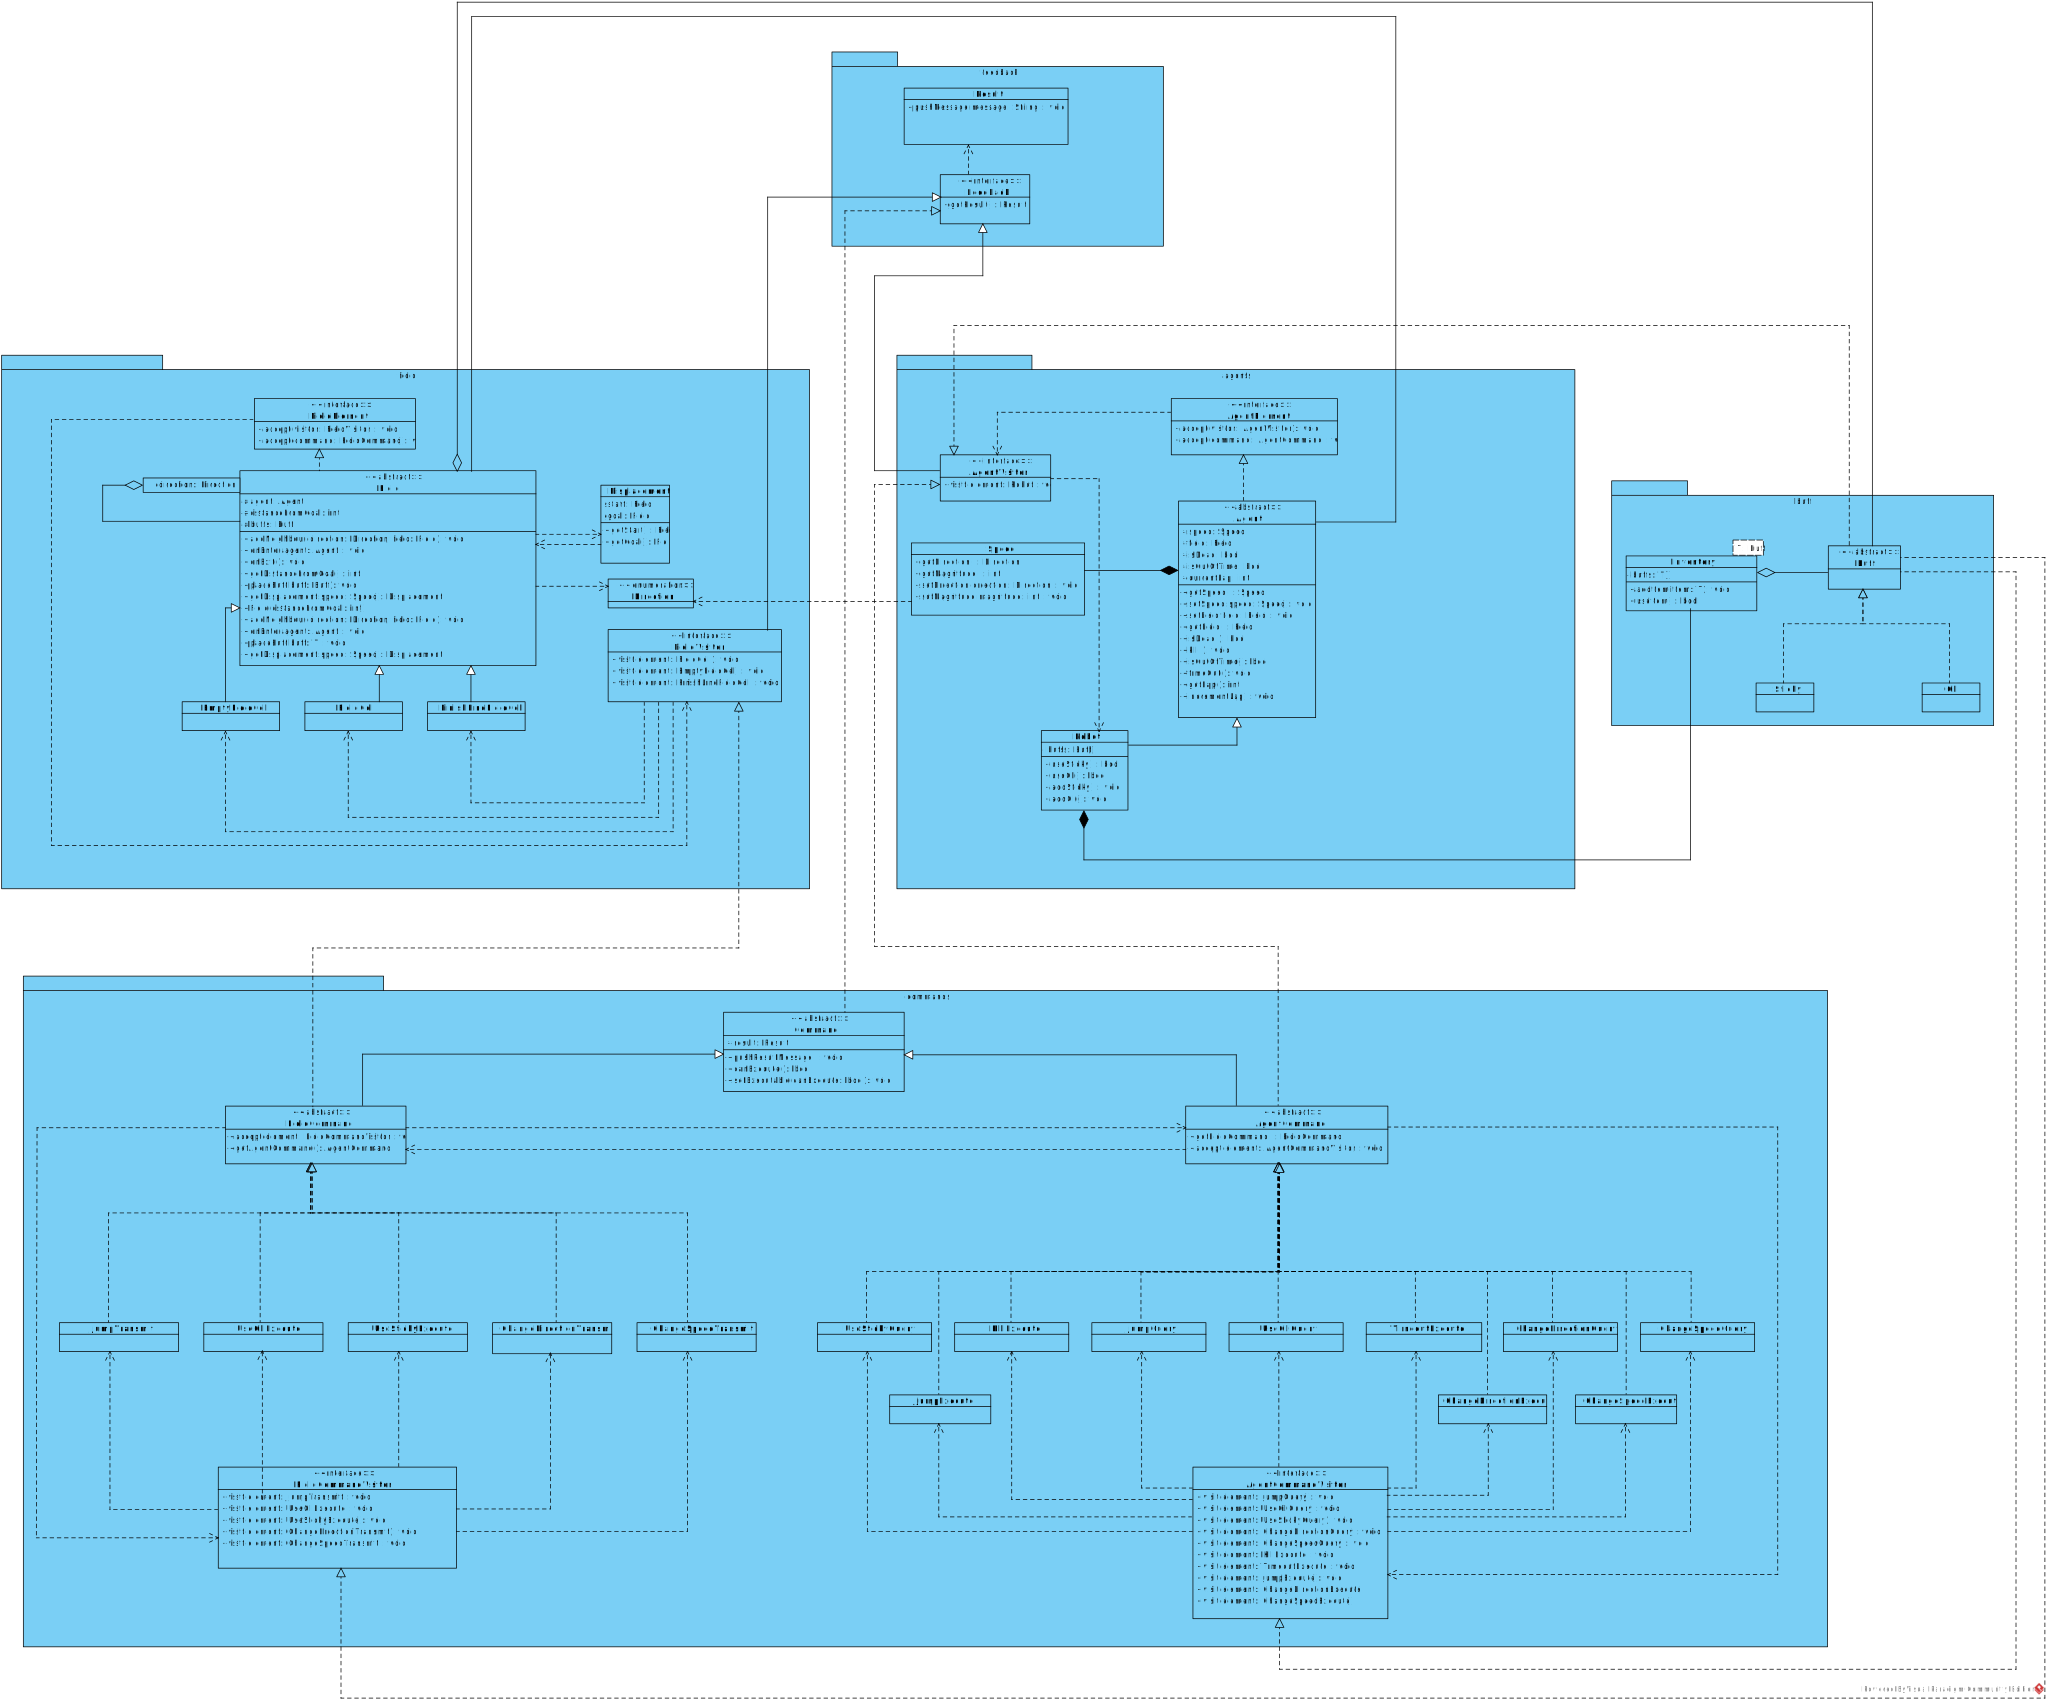
\includegraphics[width=\linewidth]{chapters/chapter03/ClassMain.pdf}
\caption{A teljes osztálydiagram}
\label{A teljes osztálydiagram}
\end{center}
\end{figure}

\begin{figure}[h]
\begin{center}
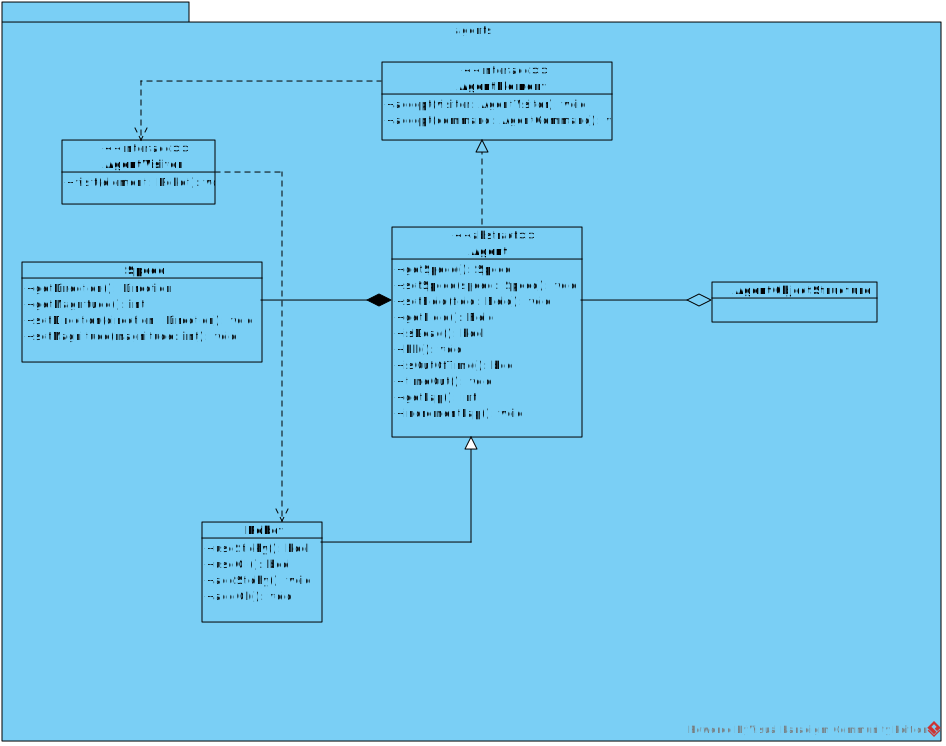
\includegraphics[width=\linewidth]{chapters/chapter03/ClassAgents.pdf}
\caption{Agents package osztálydiagram}
\label{Agents package osztálydiagram}
\end{center}
\end{figure}

\begin{figure}[h]
\begin{center}
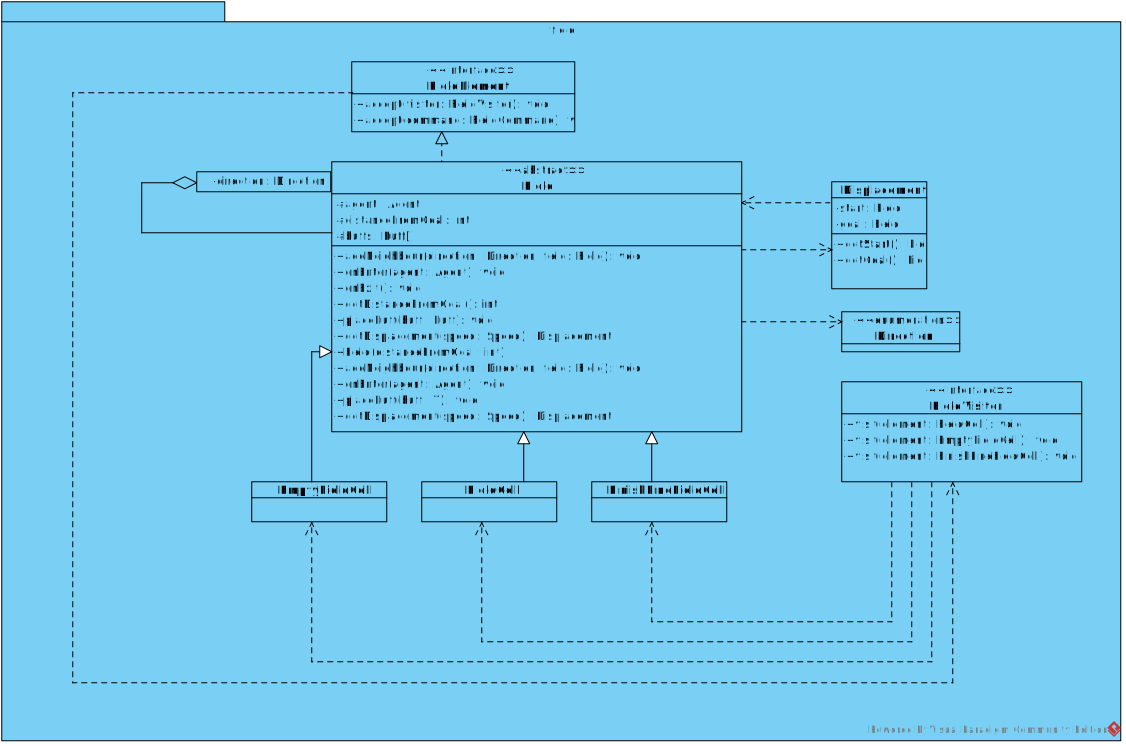
\includegraphics[width=\linewidth]{chapters/chapter03/ClassField.pdf}
\caption{Field package osztálydiagram}
\label{Field package osztálydiagram}
\end{center}
\end{figure}

\clearpage

\begin{figure}[h]
\begin{center}
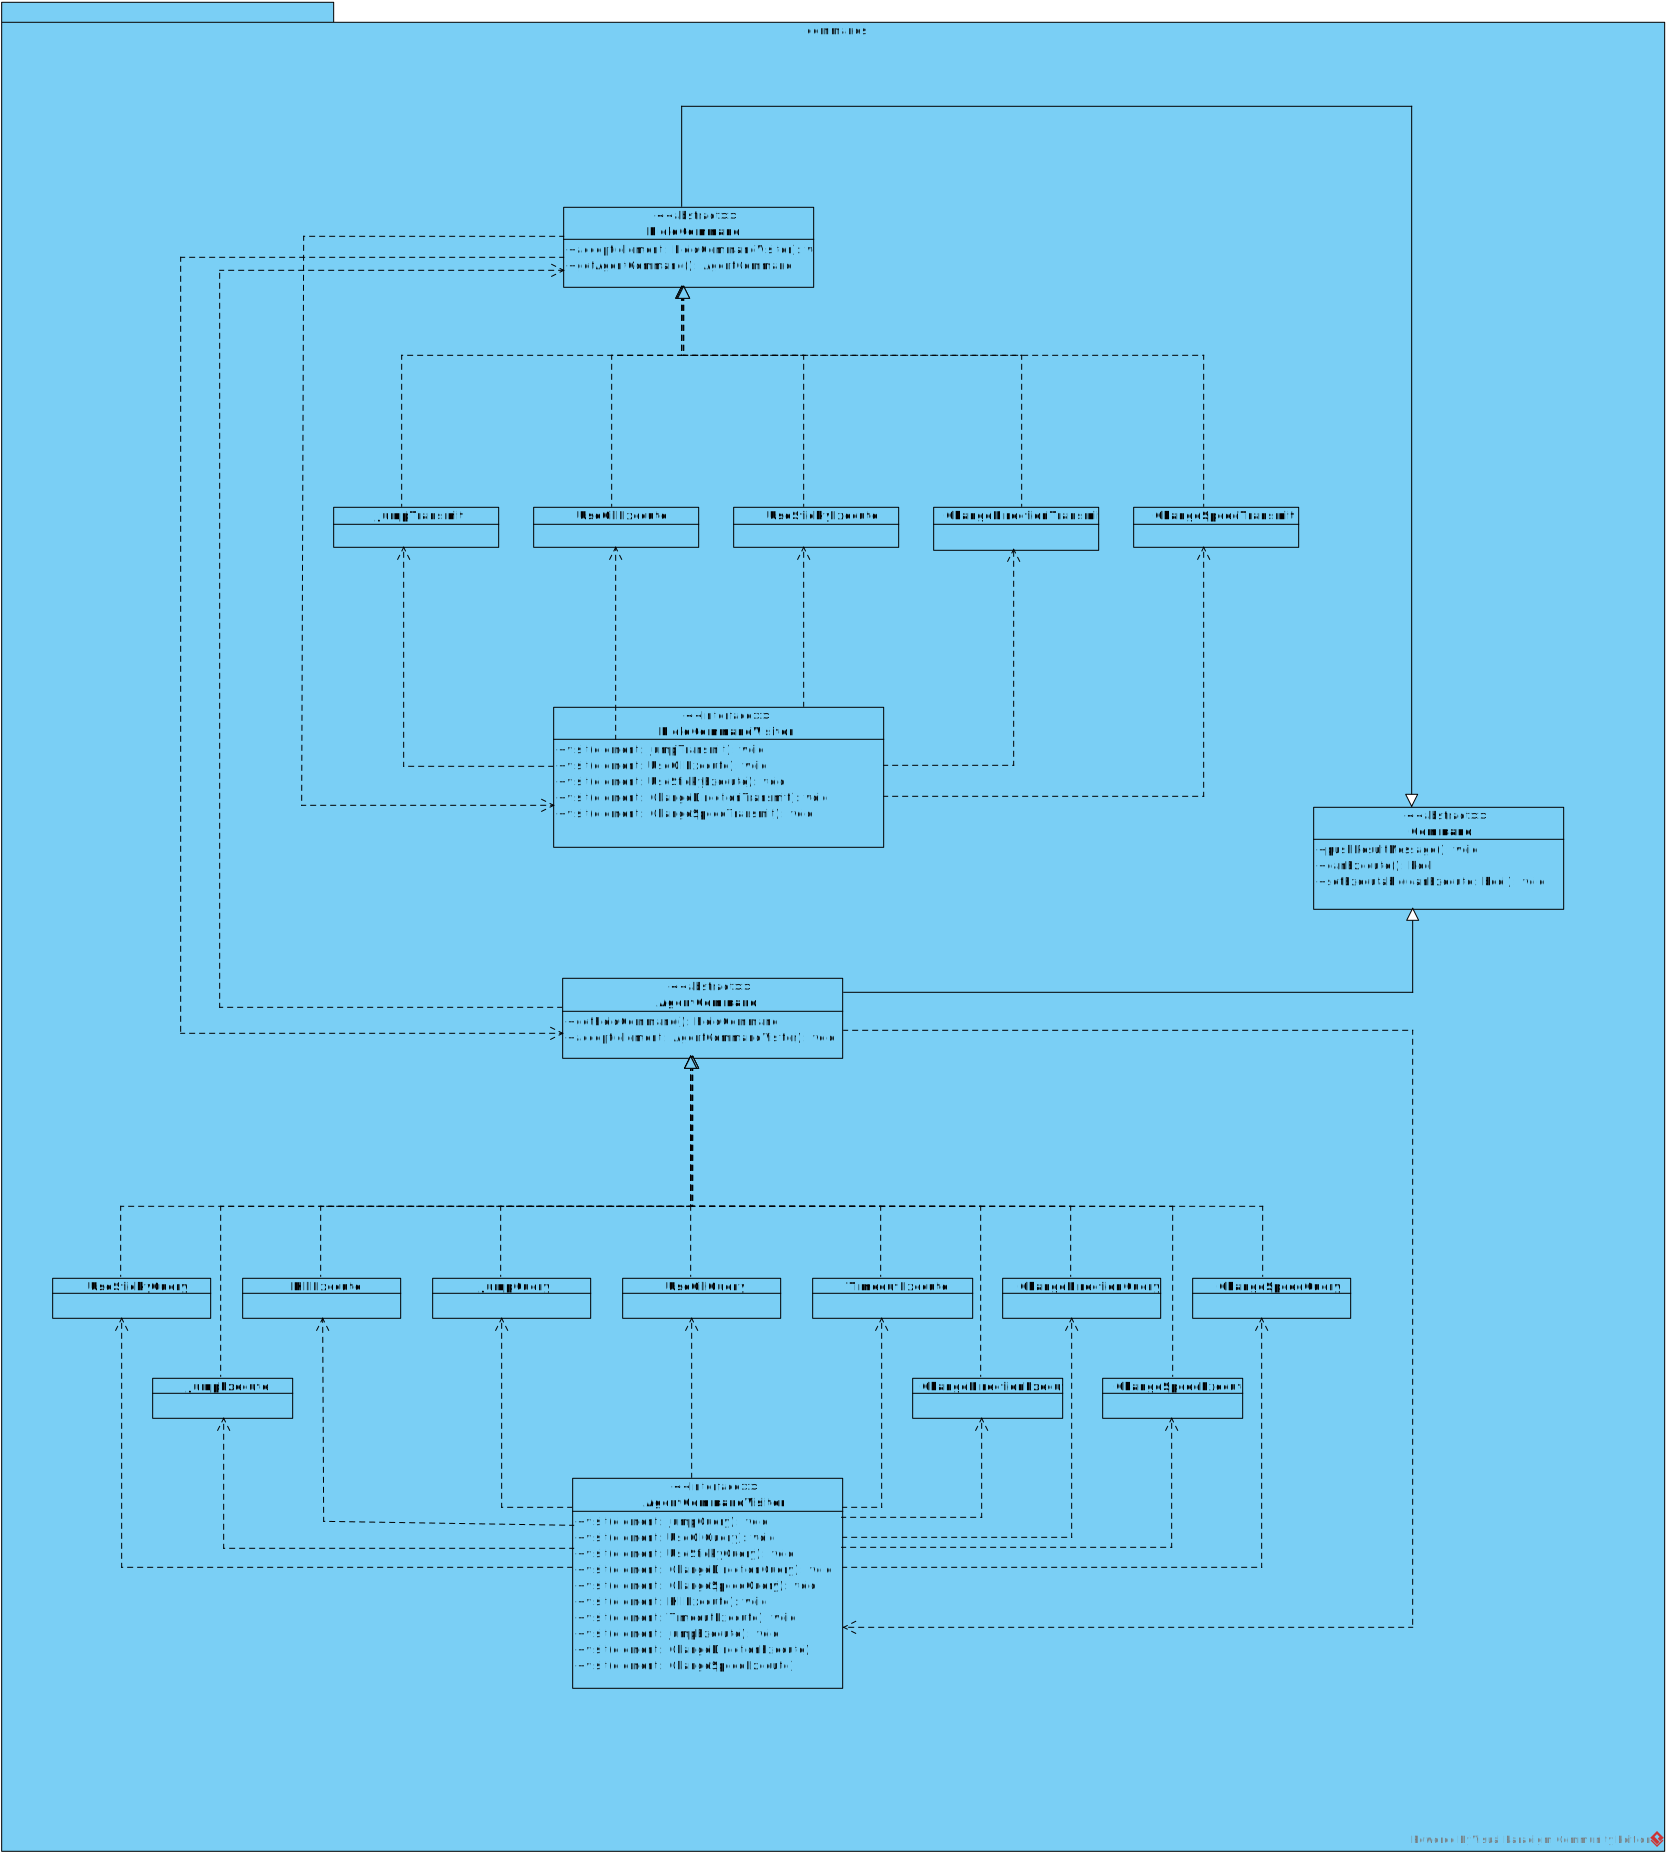
\includegraphics[width=\linewidth]{chapters/chapter03/ClassCommands.pdf}
\caption{Commands package osztálydiagram}
\label{Commands package osztálydiagram}
\end{center}
\end{figure}


\begin{figure}[h]
\begin{center}
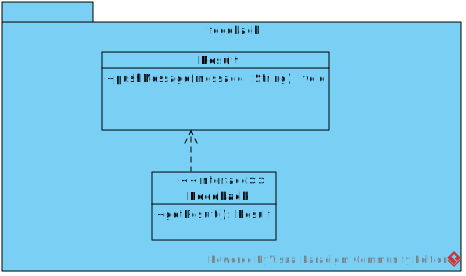
\includegraphics[width=\linewidth]{chapters/chapter03/ClassFeedback.pdf}
\caption{Feedback package osztálydiagram}
\label{Feedback package osztálydiagram}
\end{center}
\end{figure}


\begin{figure}[h]
\begin{center}
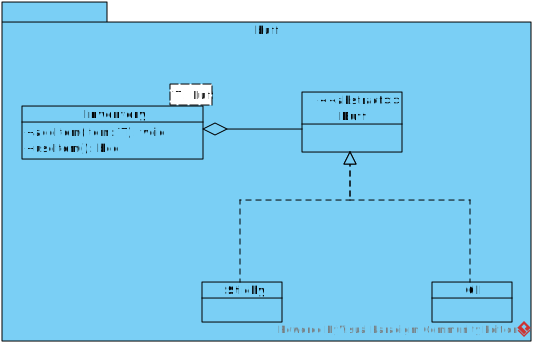
\includegraphics[width=\linewidth]{chapters/chapter03/ClassBuff.pdf}
\caption{Buff package osztálydiagram}
\label{Buff package osztálydiagram}
\end{center}
\end{figure}


\begin{figure}[h]
\begin{center}
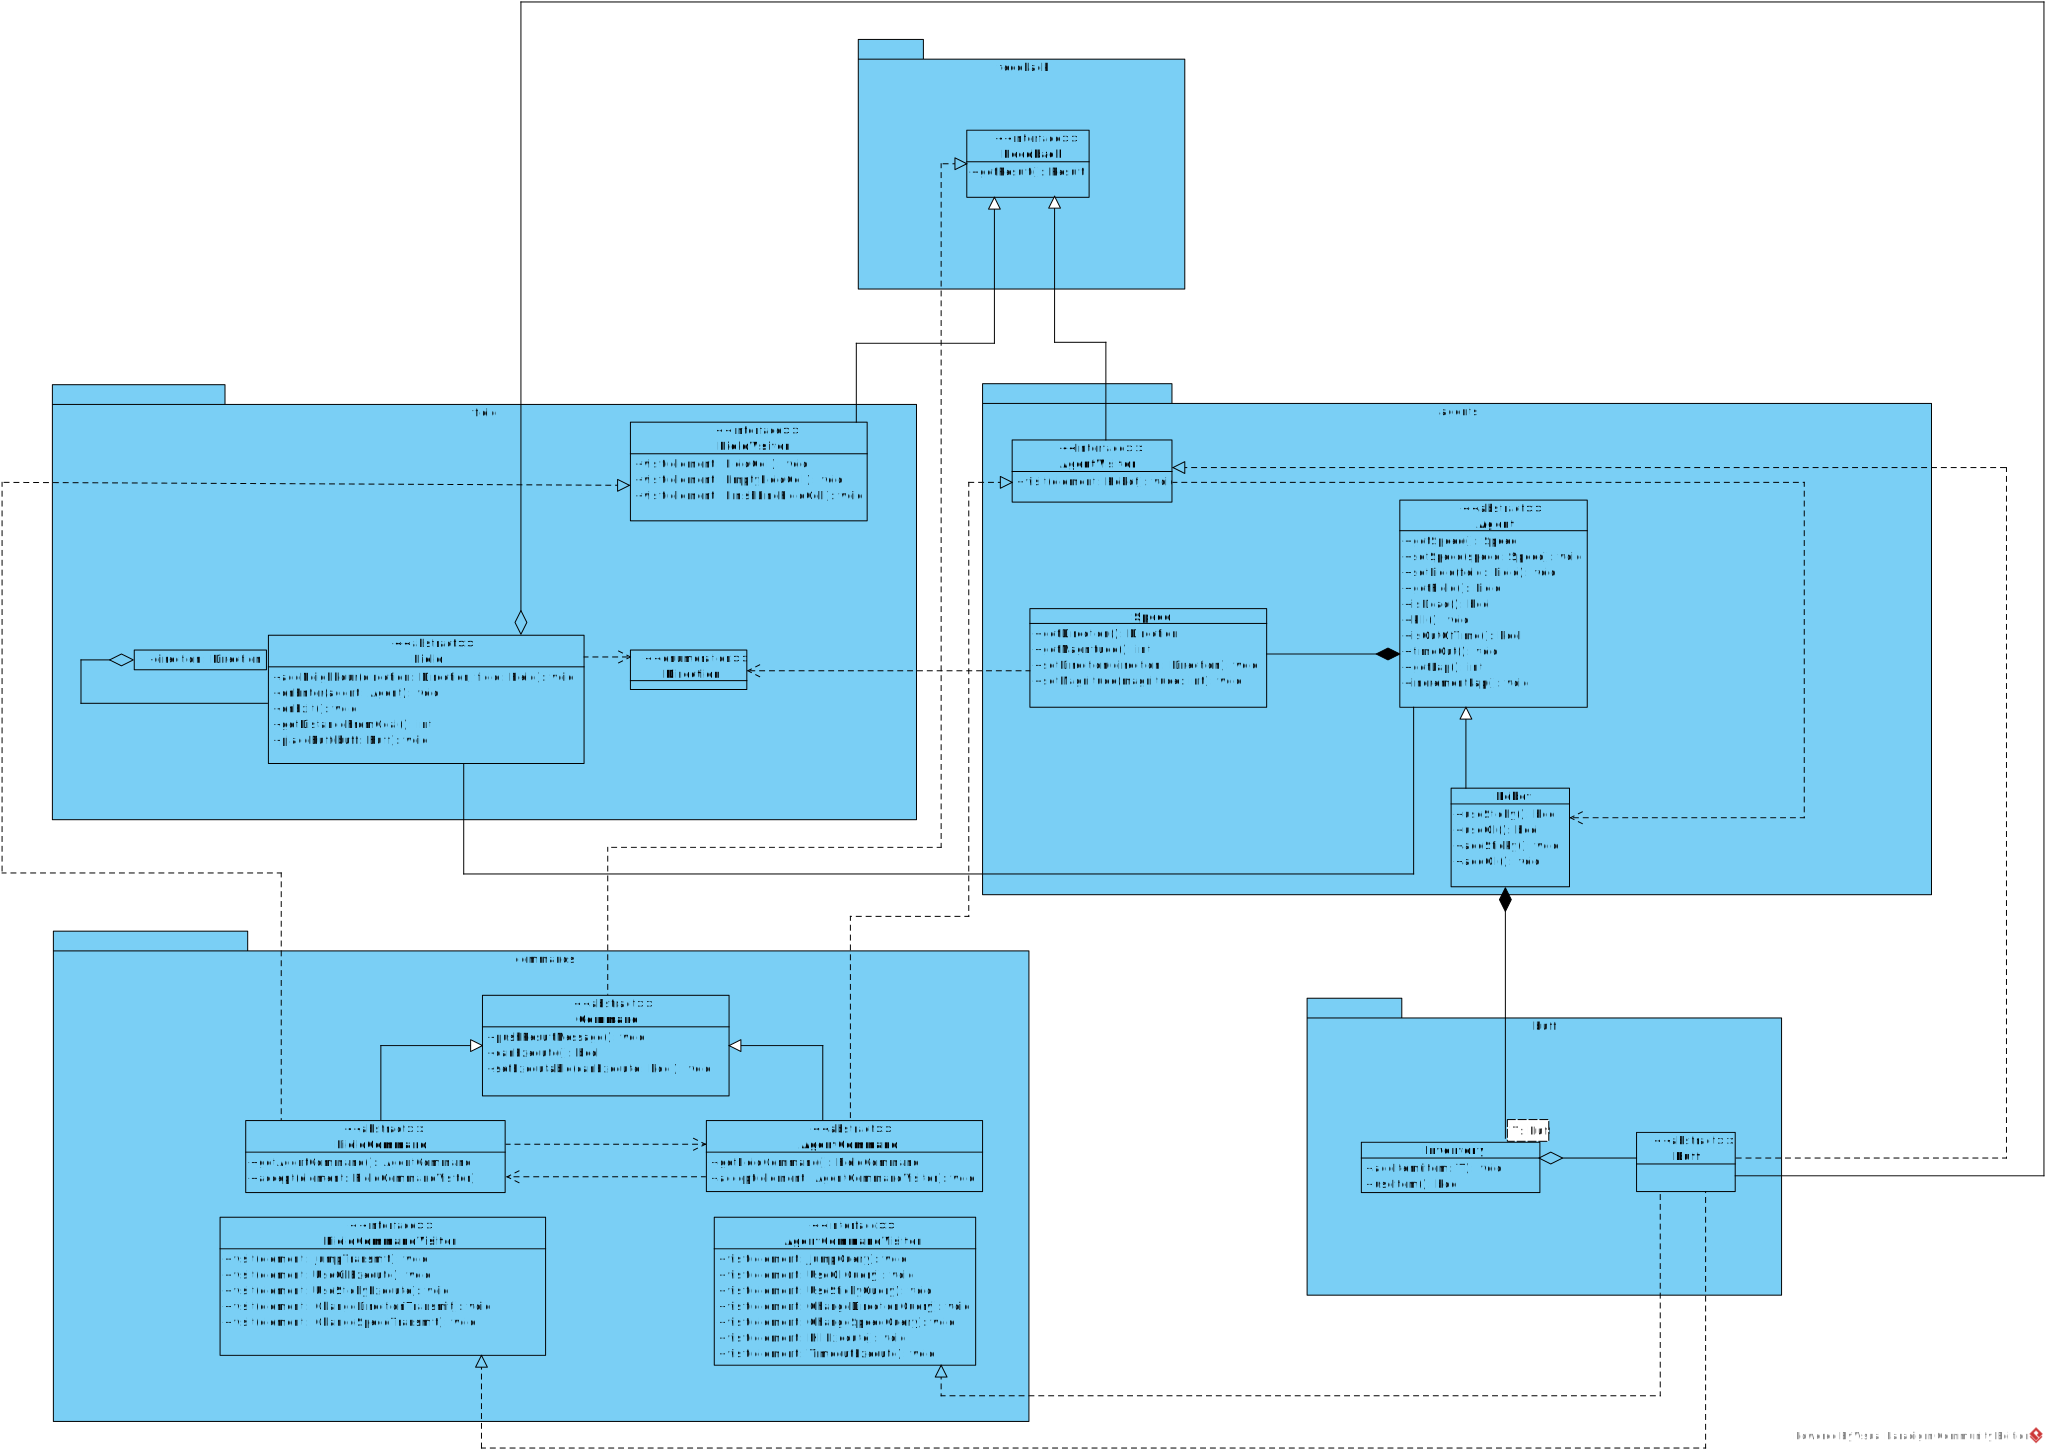
\includegraphics[width=\linewidth]{chapters/chapter03/ClassInterpackage.pdf}
\caption{Packagek közti függőségek osztálydiagramja}
\label{Packagek közti függőségek osztálydiagramja}
\end{center}
\end{figure}

\clearpage

\section{Szekvencia diagramok}

\begin{figure}[h]
	\begin{center}
		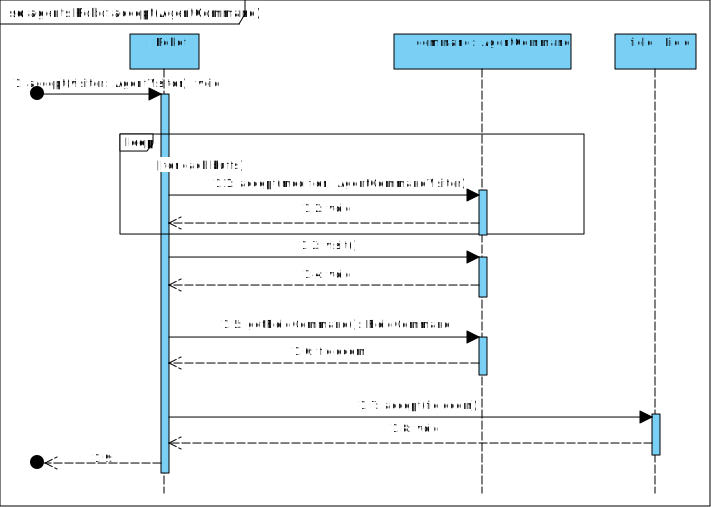
\includegraphics[width=\textwidth]{chapters/chapter03/agentsRobotacceptAgentCommand.pdf}
		\caption{Robot utasítást fogad}
		\label{fig:agents.Robot.accept}
	\end{center}
\end{figure}

\begin{figure}[h]
	\begin{center}
		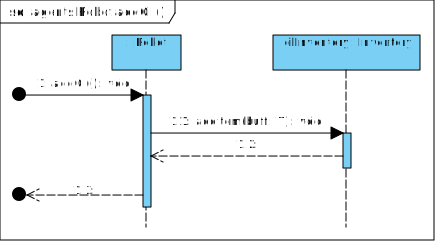
\includegraphics[width=\textwidth]{chapters/chapter03/agentsRobotaddOil.pdf}
		\caption{Robot felvesz a készletébe egy olajfoltot}
		\label{fig:agents.Robot.addOil}
	\end{center}
\end{figure}

\begin{figure}[h]
	\begin{center}
		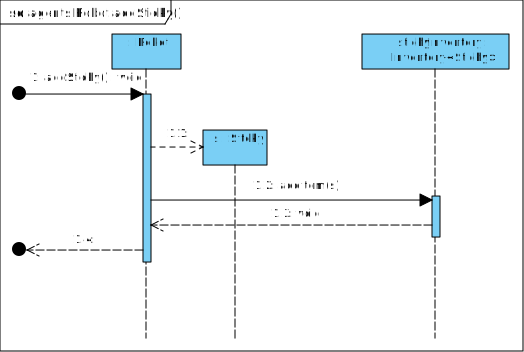
\includegraphics[width=\textwidth]{chapters/chapter03/agentsRobotaddSticky.pdf}
		\caption{Robot felvesz a készletébe egy ragacsfoltot}
		\label{fig:agents.Robot.addSticky}
	\end{center}
\end{figure}

\begin{figure}[h]
	\begin{center}
		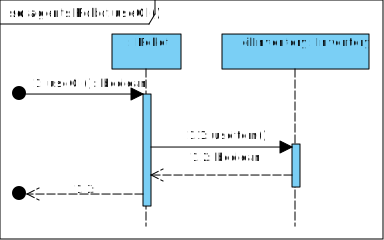
\includegraphics[width=\textwidth]{chapters/chapter03/agentsRobotuseOil.pdf}
		\caption{Robot felhasználja a készletében lévő olajfoltot ha van}
		\label{fig:agents.Robot.useOil}
	\end{center}
\end{figure}

\begin{figure}[h]
	\begin{center}
		\includegraphics[width=\textwidth]{chapters/chapter03/agentsRobotuseSticky.pdf}
		\caption{Robot felhasználja a készletében lévő ragacsfoltot ha van}
		\label{fig:agents.Robot.useSticky}
	\end{center}
\end{figure}

\begin{figure}[h]
	\begin{center}
		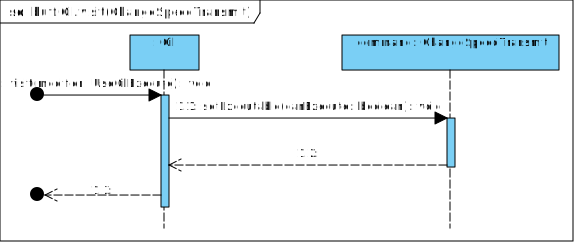
\includegraphics[width=\textwidth]{chapters/chapter03/buffOilvisitChangeSpeedTransmit.pdf}
		\caption{Olajfolt megakadályozza a sebesség nagyságának változtatását}
		\label{fig:buff.Oil.visit}
	\end{center}
\end{figure}

\begin{figure}[h]
	\begin{center}
		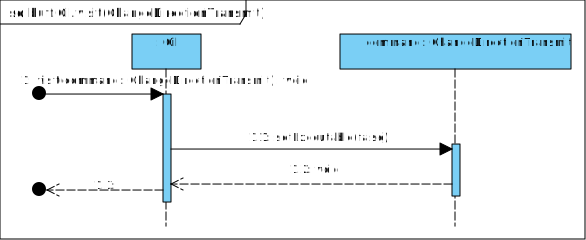
\includegraphics[width=\textwidth]{chapters/chapter03/buffOilvisitChangeDirectionTransmit.pdf}
		\caption{Olajfolt megakadályozza a sebesség irányának megváltoztatását}
		\label{fig:buff.Oil.visit2}
	\end{center}
\end{figure}

\begin{figure}[h]
	\begin{center}
		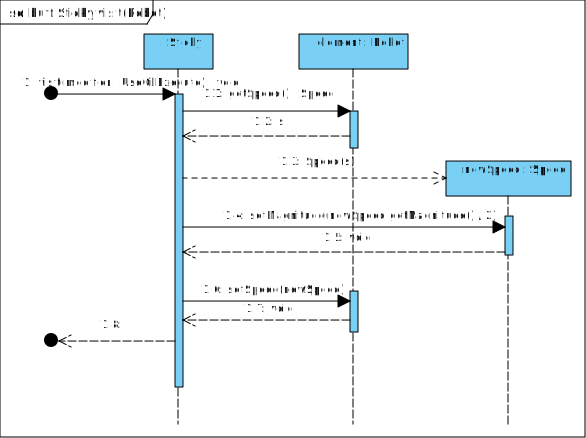
\includegraphics[width=\textwidth]{chapters/chapter03/buffStickyvisitRobot.pdf}
		\caption{Olajfolt megakadályozza a sebességváltoztatást}
		\label{fig:buff.Sticky.visit}
	\end{center}
\end{figure}

\begin{figure}[h]
	\begin{center}
		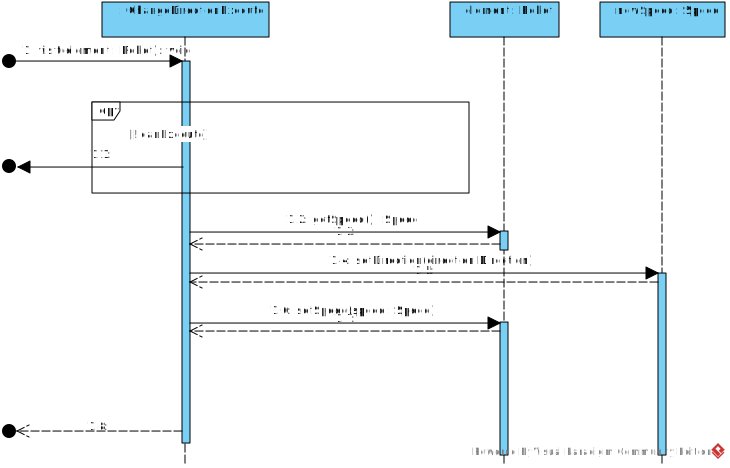
\includegraphics[width=\textwidth]{chapters/chapter03/commandsexecutesChangeDirectionExecutevisitRobot.pdf}
		\caption{Robot irányváltoztatásának végrehajtása}
		\label{fig:command.executes.ChangeDirectionExecute.visit}
	\end{center}
\end{figure}

\begin{figure}[h]
	\begin{center}
		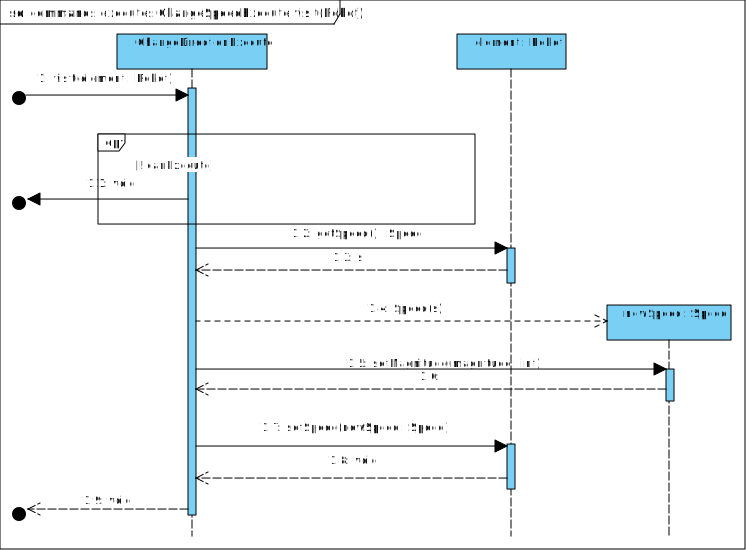
\includegraphics[width=\textwidth]{chapters/chapter03/commandsexecutesChangeSpeedExecutevisitRobot.pdf}
		\caption{Robot sebességnagyságának megváltoztatása}
		\label{fig:command.executes.ChangeSpeedExecute.visit}
	\end{center}
\end{figure}

\begin{figure}[h]
	\begin{center}
		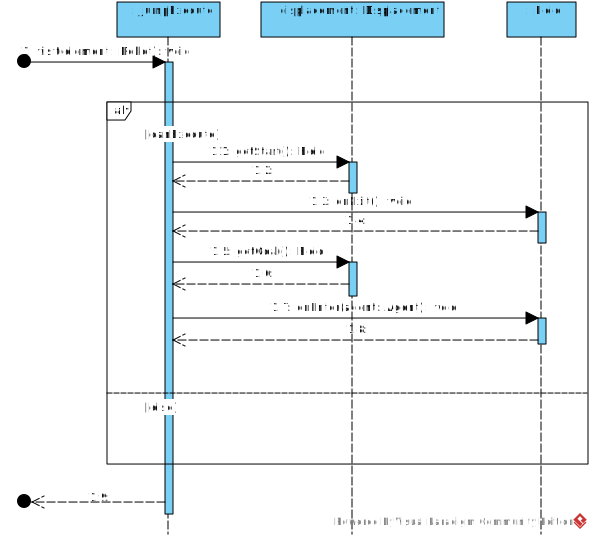
\includegraphics[width=\textwidth]{chapters/chapter03/commandsexecutesJumpExecutevisitRobot.pdf}
		\caption{Robot ugrásának végrehajtása}
		\label{fig:command.executes.JumpExecute.visit}
	\end{center}
\end{figure}

\begin{figure}[h]
	\begin{center}
		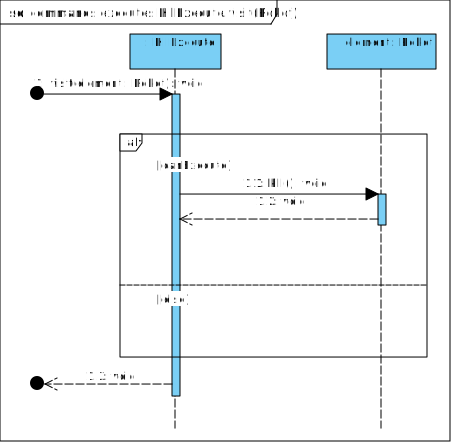
\includegraphics[width=\textwidth]{chapters/chapter03/commandsexecutesKillExecutevisitRobot.pdf}
		\caption{Robot megölésének végrehajtása}
		\label{fig:command.executes.KillExecute.visit}
	\end{center}
\end{figure}

\begin{figure}[h]
	\begin{center}
		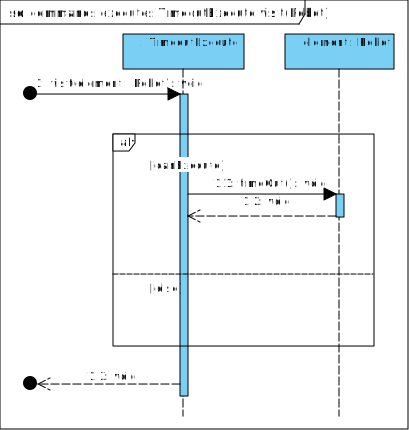
\includegraphics[width=\textwidth]{chapters/chapter03/commandsexecutesTimeoutExecutevisitRobot.pdf}
		\caption{Robot idő lejártának végrehajtása}
		\label{fig:command.executes.TimeoutExecute.visit}
	\end{center}
\end{figure}

\begin{figure}[h]
	\begin{center}
		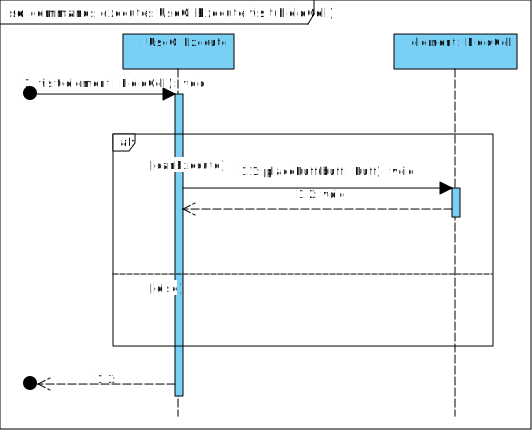
\includegraphics[width=\textwidth]{chapters/chapter03/commandsexecutesUseOilExecutevisitFieldCell.pdf}
		\caption{Robot lehelyezi az Olaj foltot a mezőre}
		\label{fig:command.executes.UseOilExecute.visit}
	\end{center}
\end{figure}

\begin{figure}[h]
	\begin{center}
		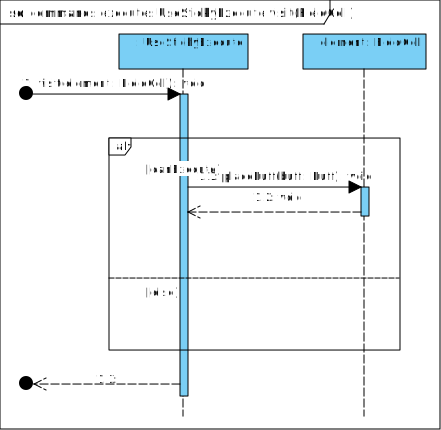
\includegraphics[width=\textwidth]{chapters/chapter03/commandsexecutesUseStickyExecutevisitFieldCell.pdf}
		\caption{Robot lehelyezi a Ragacs foltot a mezőre}
		\label{fig:command.executes.UseStickyExecute.visit}
	\end{center}
\end{figure}

\clearpage

\begin{figure}[h]
	\begin{center}
		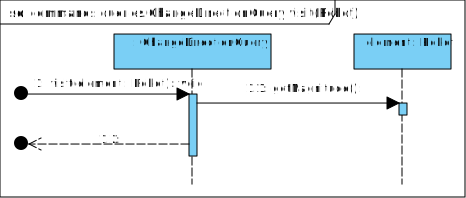
\includegraphics[width=\textwidth]{chapters/chapter03/commandsqueriesChangeDirectionQueryvisitRobot.pdf}
		\caption{Robot irányváltásra való felkérése}
		\label{fig:command.executes.ChangeDirectionQuery.visit}
	\end{center}
\end{figure}

\begin{figure}[h]
	\begin{center}
		\includegraphics[width=\textwidth]{chapters/chapter03/commandsqueriesChangeSpeedQueryvisitRobot.pdf}
		\caption{Robot sebesség nagyságának megváltoztatására való felkérése}
		\label{fig:command.executes.ChangeSpeedQuery.visit}
	\end{center}
\end{figure}

\begin{figure}[h]
	\begin{center}
		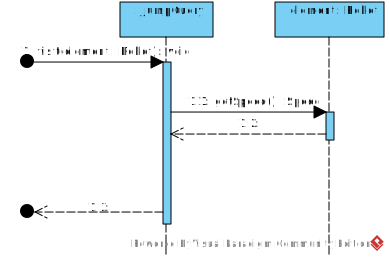
\includegraphics[width=\textwidth]{chapters/chapter03/commandsqueriesJumpQueryvisitRobot.pdf}
		\caption{Robot ugrásra azaz helyzetmódosításra való felkérése}
		\label{fig:command.executes.JumpQuery.visit}
	\end{center}
\end{figure}

\begin{figure}[h]
	\begin{center}
		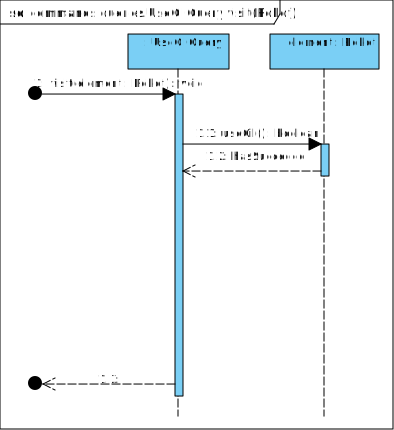
\includegraphics[width=\textwidth]{chapters/chapter03/commandsqueriesUseOilQueryvisitRobot.pdf}
		\caption{Robotot Olaj lehelyezésére való felkérése}
		\label{fig:command.executes.UseOilQuery.visit}
	\end{center}
\end{figure}

\begin{figure}[h]
	\begin{center}
		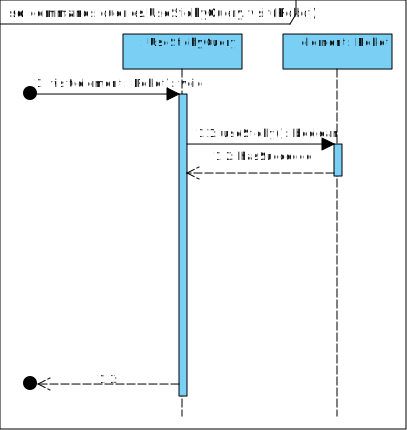
\includegraphics[width=\textwidth]{chapters/chapter03/commandsqueriesUseStickyQueryvisitRobot.pdf}
		\caption{Robotot Ragacs lehelyezésére való felkérése}
		\label{fig:command.executes.UseStickyQuery.visit}
	\end{center}
\end{figure}

\begin{figure}[h]
	\begin{center}
		\includegraphics[width=\textwidth]{chapters/chapter03/commandstransmitsChangeDirectionTransmitvisitFieldCell.pdf}
		\caption{Irányváltásra vonatkozó kérés átvitele}
		\label{fig:command.executes.ChangeDirectionTransmit.visit}
	\end{center}
\end{figure}

\begin{figure}[h]
	\begin{center}
		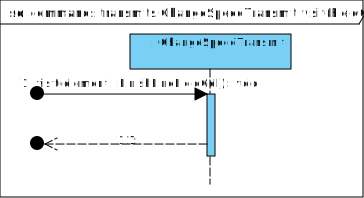
\includegraphics[width=\textwidth]{chapters/chapter03/commandstransmitsChangeSpeedTransmitvisitFieldCell.pdf}
		\caption{Szebességnagyság változtatásra vonatkozó kérés átvitele}
		\label{fig:command.executes.ChangeSpeedTransmit.visit}
	\end{center}
\end{figure}

\begin{figure}[h]
	\begin{center}
		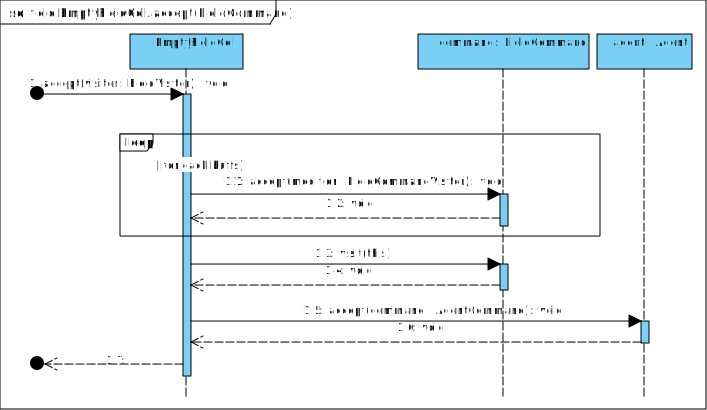
\includegraphics[width=\textwidth]{chapters/chapter03/fieldEmptyFieldCellacceptFieldCommand.pdf}
		\caption{Üres pályamező utasításfeldolgozása}
		\label{fig:field.EmptyFieldCell.accept}
	\end{center}
\end{figure}

\begin{figure}[h]
	\begin{center}
		\includegraphics[width=\textwidth]{chapters/chapter03/fieldFieldCellacceptFieldCommand.pdf}
		\caption{Pályamező utasításfeldolgozása}
		\label{fig:field.FieldCell.accept}
	\end{center}
\end{figure}

\begin{figure}[h]
	\begin{center}
		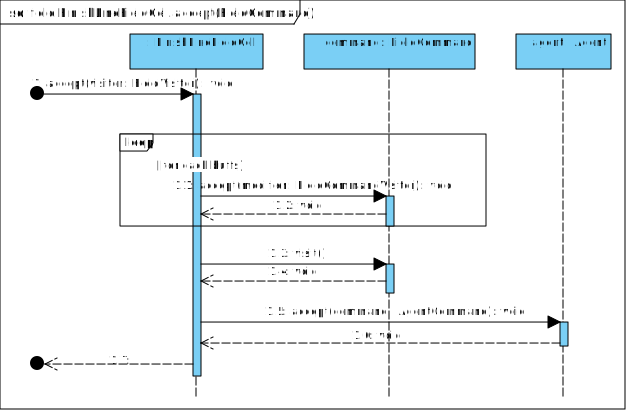
\includegraphics[width=\textwidth]{chapters/chapter03/fieldFinishLineFieldCellacceptFieldCommand.pdf}
		\caption{Start/célvonal pályamező utasításfeldolgozása}
		\label{fig:field.FinishLineFieldCell.accept}
	\end{center}
\end{figure}

\clearpage

\section{State-chartok}
\comment{Csak azokhoz az osztályokhoz, ahol van értelme. Egyetlen állapotból álló state-chartok ne szerepeljenek. A játék működését bemutató state-chart-ot készíteni tilos.}

\begin{figure}[h]
\begin{center}
%\includegraphics[width=17cm]{chapters/chapter03/example.pdf}
\caption{x}
\label{fig:example3}
\end{center}
\end{figure}


%% Szglab4
% ===========================================================================
%
\section{Napló}

\begin{naplo}

\bejegyzes
{2015.02.25. ~8.00}
{2 óra}
{Nagy} 
{Tevékenység: Elkészíti a Konzultációs jegyzőkönyvet.\newline } 

\bejegyzes
{2015.02.15 ~19.00}
{1 óra}
{Nagy} 
{Nagy előkészíti a feladatokat, felveszi őket a GitHub-ra..} 

\bejegyzes
{2015.02.25 ~20.00}
{2 óra}
{Paral \newline Nyári \newline Szőke \newline Nagy} 
{Értekezlet.
Döntés: Feladatok felosztása az feladatok hozzárendelése a megfelelő emberekhez. A részletek megbeszélése, tervezés, koncepciók átgondolása.\newline } 

\bejegyzes
{2015.02.26. ~20.00}
{1 óra}
{Paral \newline Nyári \newline Szőke \newline Nagy} 
{Értekezlet.
Döntés: Általános megbeszélés, előrehaladás ellenőrzése. A felmerülő problémák azonosítása és eliminálása. \newline } 

\bejegyzes
{2015.02.27. ~19.00}
{2 óra}
{Paral \newline Nyári \newline Szőke \newline Nagy} 
{Értekezlet.
Döntés: Elkészült tervek átnézése, lehetséges jövőbeli problémák azonosítása az architektúrával kapcsolatban. Hátralévő feladatok azonosítása.\newline } 

\bejegyzes
{2015.02.27. ~21.00}
{1 óra}
{Paral \newline Nyári \newline Szőke \newline Nagy} 
{Értekezlet.
Döntés: Elkészült tervek utolsó átnézése, apróbb módosítások kiosztása.\newline } 

\bejegyzes
{2015.02.26. ~17.00}
{5 óra}
{Paral} 
{Tevékenység: Statikus struktúra diagrammok szekció elkészítése.\newline } 

\bejegyzes
{2015.02.27. ~8.00}
{2 óra}
{Nyári} 
{Tevékenység: Statikus struktúra diagrammok szekcióban apróbb módosítások eszközölése.\newline } 

\bejegyzes
{2015.02.27. ~13.00}
{2 óra}
{Szőke} 
{Tevékenység: Statikus struktúra diagrammok szekcióban apróbb módosítások eszközölése.\newline } 

\bejegyzes
{2015.02.25. ~21.00}
{2 óra}
{Paral} 
{Tevékenység: Objektumkatalógus szekció elkészítése.\newline } 

\bejegyzes
{2015.02.25. ~21.00}
{5 óra}
{Nyári} 
{Tevékenység: Szekvenciadiagrammok szekció elkészítése.\newline } 

\bejegyzes
{2015.02.26. ~15.00}
{2 óra}
{Szőke} 
{Tevékenység: További szekvenciadiagrammok szekció elkészítése.\newline } 

\bejegyzes
{2015. 02.28. ~10.00}
{1 óra}
{Nagy}
{Tevékenység: Osztályleírások elkészítése.\newline }

\bejegyzes
{2015.02.28. ~12.00}
{1 óra}
{Paral}
{Tevékenység: Osztályleírások átnézése, finomítása.\newline}

\bejegyzes
{2015.02.28. ~16.00}
{30 perc}
{Nyári}
{Tevékenység:  State Chart diagramok elkészítése}

\bejegyzes
{2015.02.28 ~17.00}
{1 óra}
{Paral} 
{Tevékenység: Reviewra szánt idő a pull-requestekre.\newline } 

\bejegyzes
{2015.02.28. ~17.00}
{1 óra}
{Nyári} 
{Tevékenység: Reviewra szánt idő a pull-requestekre.\newline } 

\bejegyzes
{2015.02.28. ~17.00}
{1 óra}
{Szőke} 
{Tevékenység: Reviewra szánt idő a pull-requestekre.\newline } 

\bejegyzes
{2015.02.28. ~17.00}
{1 óra}
{Nagy} 
{Tevékenység: Reviewra szánt idő a pull-requestekre.\newline } 

\bejegyzes
{2015.03.1. ~8.00}
{1 óra}
{Nagy} 
{Tevékenység: Követelmények, projekt, funckionalitás leadandó módosításainak hozzáadása.\newline } 

\bejegyzes
{2015.03.1. ~10.00}
{1 óra}
{Nagy} 
{Tevékenység: Napló elkészítése.\newline } 

\end{naplo}



%\setcounter{chapter}{3}
%\input{chapters/chapter04/sablon04}
%% Szglab4
% ===========================================================================
%
\section{Napló}

\begin{naplo}
	
	\bejegyzes
	{2015.03.04. ~8.00}
	{2 óra}
	{Nyári} 
	{Tevékenység: Elkészíti a Konzultációs jegyzőkönyvet.\newline } 
	
	
	\bejegyzes
	{2015.03.04 ~20.00}
	{2 óra}
	{Paral \newline Nyári \newline Szőke \newline Nagy} 
	{Értekezlet.
		Döntés: Feladatok felosztása az feladatok hozzárendelése a megfelelő emberekhez. A részletek megbeszélése, tervezés, koncepciók átgondolása.\newline } 
			
	
	\bejegyzes
	{2015.03.07. ~08.00}
	{4 óra}
	{Szőke} 
	{Tevékenység: Szekvenciadiagrammok szekció javítása.\newline } 
		
	\bejegyzes
	{2015.03.08 ~17.00}
	{1 óra}
	{Nagy} 
	{Tevékenység: Reviewra szánt idő a pull-requestekre.\newline } 
	
	\bejegyzes
	{2015.03.08. ~17.00}
	{1 óra}
	{Nyári} 
	{Tevékenység: Reviewra szánt idő a pull-requestekre.\newline } 
			
	\bejegyzes
	{2015.03.08. ~10.00}
	{1 óra}
	{Szőke} 
	{Tevékenység: Napló elkészítése.\newline } 
	
\end{naplo}





%\setcounter{chapter}{4}
%% Szglab4
% ===========================================================================
%
\chapter{Szkeleton tervezése}

\thispagestyle{fancy}

\section{A szkeleton modell valóságos use-case-ei}
\comment{A szkeletonnak, mint önálló programnak a működésével kapcsolatos use-case-ek.}

\subsection{Use-case diagram}

\begin{figure}[h]
\begin{center}
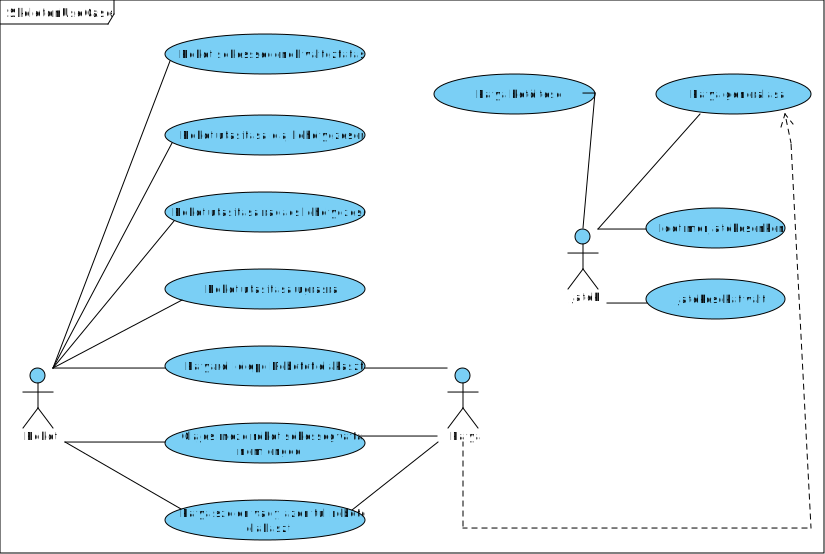
\includegraphics[width=\textwidth]{chapters/chapter05/SkeletonUseCase.pdf}
\caption{Szkeleton Use Case Diagram}
\label{fig:SzkeletonUseCase}
\end{center}
\end{figure}

\subsection{Use-case leírások}
%\comment{Minden use-case-hez külön}

\usecase%
{Új játék indítása}%
{Elindíthatunk egy új játékot}%
{Játékos, Játék}%
{A játékosok számának megadása után a Játékos kezdeményezheti a játéknak az elindítását}

\usecase%
{Játék megnyerése}%
{Játék végső helyzete alapján győztes eldöntése}%
{Játékos, Játék}%
{Ha minden Játékosnak lejár akkor a megtett út alapján eldől, hogy ki a győztes}

\usecase%
{Játék elvesztése}%
{Játék végső helyzete alapján vesztesek eldöntése}%
{Játékos, Játék}%
{Ha minden Játékosnak lejár akkor a megtett út alapján eldől, hogy kik a vesztesek}

\usecase%
{Játékparaméterek megadása}%
{Új játék paramétereinek megadása}%
{Játék}%
{Játékosok megadhatják, hogy hányan vannak, milyen időkorláttal kívánnak játszani}

\usecase%
{Pálya generálása}%
{Új játékpályát generálunk}%
{Játék, Játékos}%
{A Játékosok egy új pályát kívánnak generálni}

\usecase%
{Pálya beltöltése}%
{Előre elkészített pályát töltünk be}%
{Játék, Játékos}%
{Ha a játékosok nem véletlenszerű pályán akarnak játszani}

\usecase%
{Pálya beltöltése}%
{Előre elkészített pályát töltünk be}%
{Játék, Játékos}%
{Ha a játékosok nem véletlenszerű pályán akarnak játszani}

\usecase%
{Jelenlegi játék mentése}%
{Játék aktuállis állásának mentése}%
{Játék, Játékos}%
{A Játékosok valamilyen oknál kifolyólag később akarják folytatni a játékot}

\usecase%
{Mentett játék betöltáse}%
{Már elmentett jűték betöltése}%
{Játék, Játékos}%
{A Játékosok a régebben félbehagyott játékot folytathatják ahol abbahagyták}

\usecase%
{Időt mér játékosonkét}%
{Játékmenet és Játékosonkénti időnyilvántartás}%
{Játék}%
{Nyilvántartja a Játékosok még hátralévő idejét, és megállítja azokat akik már nem képhetnek}

\usecase%
{Játékosokat vált}%
{Játékosokat vált körönként}%
{Játék}%
{Játékost cserél körönként ha a játékos ugrott vagy lejárt az ideje}

\usecase%
{Robot sebességének változtatása}%
{A Játékos megváltoztathatja a Robotnak a sebességét}%
{Játékos, Robot}%
{A játékos körönként megváltoztathatja a Robotnak a sebességét}

\usecase%
{Robot utasítása olajnak a lehelyezése}%
{Játékos utasíthatja a Robotot, hogy helyezze le az olajfoltot}%
{Játékos, Robot}%
{A Játékos más játékosok hátráltatásának okán lehelyezhet a készletáéből egy olajfoltot}

\usecase%
{Robot utasítása ragacsnak a lehelyezése}%
{Játékos utasíthatja a Robotot, hogy helyezze le az ragacsfoltot}%
{Játékos, Robot}%
{A Játékos más játékosok hátráltatásának okán lehelyezhet a készletáéből egy ragacsfoltot}

\usecase%
{Robot utasítása ugrásra}%
{Játékos utasíthatja a Robotot, hogy végezze el az ugrást}%
{Játékos, Robot, Játék}%
{Játékos utasíthatja a Robotot, hogy végezze el az ugrást, amennyiben ezt nem teszi meg a Játék kikényszerítheti ezt a lépést}

\usecase%
{Olajos mező Robot sebességváltoztatást nem enged}%
{Ha olajos mezőn vagyunk akkor a mező nem engedi a lépést a robotnak}%
{Robot, Pálya}%
{Ha egy Robot rálép az olajra akkor a mező nem engedi neki a sebességváltoztatást}

\usecase%
{Ragacs mező Robot sebességet megfelez}%
{Ha ragacsos mezőn vagyunk akkor a mező megfelezi a Robot sebességét}%
{Robot, Pálya}%
{Ha egy Robot rálép a ragacsra akkor a mező megfelezi aa Robotnak a sebességét}

\usecase%
{Pályáról lelépő Robotot elakaszt}%
{Pályáról lelépő robotot elakasztjuk, nem léphet tovább}%
{Robot, Pálya}%
{Ha egy Robot kilép a pálya határain kívülre akkor elakasztja őt}

\section{A szkeleton kezelői felületének terve, dialógusok}
A szkeleton menüvezérléssel teszi lehetővé a különböző funckiók tesztelését. Egy teszt futtatásához szükséges a felhsználónak
megadni a tesztesetet, melyet futtatni kíván. 

A menü felépítése: \\

Példa:
1. [Use-case neve] \\
1.1 [Teszteset neve][Visszatérése] \\
1.2 [Teszteset neve][Visszatérése] \\
1.3 [Teszteset neve][Visszatérése] \\
   1.3.1 [Teszteset neve][Visszatérése] \\
... \\

Az egyes tesztesetek nevei az első pontban leírt use-casek. A tesztesetek pedig
az adott use-case összes szekvenciáját végrehajtják, amennyiben azt a felhasználó igényli. \\

A kimenet felépítése: \\

Példa: \\

Adja meg a végrehajtandó Use-case számát: X \\
X. [Use-case neve] \\
>   <osztály::függvénynév(paraméter)> \\
>         <osztály::függvénynév(paraméter)> \\
>               <osztály::függvénynév(paraméter)> \\
.                    [Teszteset neve][Értéke] \\
<               <osztály::függvénynév(paraméter)> \\
<         <osztály::függvénynév(paraméter)> \\
<   <osztály::függvénynév(paraméter)> \\

A fenti példában a > szimbólum jelzi egy függvény meghívását, < pedig egy függvény
visszatérését. A . szimbólum valamely teszteset lefutását mutatja, mely után annak 
visszatérési értéke is látszik, jelezvén, hogy sikeresen lefutott-e. \\


\section{Szekvencia diagramok a belső működésre}
\comment{A szkeletonban implementált szekvenciadiagramok. Tipikusan egy use-case egy diagram. Ezek megegyezhetnek a korábban specifikált diagramokkal, de az egyes életvonalakat (lifeline) egyértelműen a szkeletonban példányosított objektumokhoz kell tudni kötni. Azt kell megjeleníteni, hogy a szkeletonban létrehozott objektumok egymással hogyan fognak kommunikálni.}

\section{Kommunikációs diagramok}
\comment{A szkeletonban, az egyes szkeleton-use-case-ek futása során létrehozott objektumok és kapcsolataik bemutatására szolgáló diagramok. Ezek alapján valósítják meg a szkeleton fejlesztői az inicializáló kódrészleteket.}

%% Szglab4
% ===========================================================================
%
\section{Napló}

\begin{naplo}
	
	\bejegyzes
	{2015.03.11. ~8.00}
	{2 óra}
    {Szőke} 
	{Tevékenység: Elkészíti a Konzultációs jegyzőkönyvet.\newline } 
	
	\bejegyzes
	{2015.03.11 ~20.00}
	{2 óra}
	{Paral \newline Nyári \newline Szőke \newline Nagy} 
	{Értekezlet.
		Döntés: Feladatok felosztása az feladatok hozzárendelése a megfelelő emberekhez. A részletek megbeszélése, tervezés, koncepciók átgondolása.\newline } 
			
	
	\bejegyzes
	{2015.03.12. ~20.00}
	{4 óra}
	{Szőke} 
	{Tevékenység: Szekvenciadiagrammok belső működése szekció elkészítése.\newline } 
		
	\bejegyzes
	{2015.03.12. ~20.00}
	{1 óra}
	{Nagy} 
	{Tevékenység: A szkeleton felületének terve, belső dialógusok szekció elkészítése.\newline } 
		
    	
	\bejegyzes
	{2015.03.12. ~20.00}
	{2 óra}
	{Nyári} 
	{Tevékenység: Kommunikáció diagrammok szekció elkészítése.\newline } 
		
    
    \bejegyzes
    {2015.03.12. ~20.00}
    {3 óra}
    {Nyári} 
    {Tevékenység: A szkeleton modell valóságos use-caseinek elkészítése.\newline } 
        
    \bejegyzes
    {2015.03.12. ~22.00}
    {2 óra}
    {Paral} 
    {Tevékenység: A szkeleton modell valóságos use-caseinek javítása.\newline } 

    \bejegyzes
    {2015.03.12. ~23.00}
    {1 óra}
    {Nagy} 
    {Tevékenység: A szkeleton modell valóságos use-caseinek átnézése.\newline } 

    \bejegyzes
	{2015.03.15 ~20.00}
	{1 óra}
	{Nagy} 
	{Tevékenység: Reviewra szánt idő a pull-requestekre.\newline } 
	
	\bejegyzes
	{2015.03.15. ~17.00}
	{1 óra}
	{Paral} 
	{Tevékenység: Reviewra szánt idő a pull-requestekre.\newline } 
			
	\bejegyzes
	{2015.03.15. ~23.00}
	{1 óra}
	{Nagy} 
	{Tevékenység: Napló elkészítése.\newline } 
	
\end{naplo}





\setcounter{chapter}{5}
% Szglab4
% ===========================================================================
%
\chapter{Szkeleton beadás}

\thispagestyle{fancy}

\section{Fordítási és futtatási útmutató}
\begin{tabularx}{\linewidth}{| l | l | l | X |}
\hline
\textbf{Fájl neve} & \textbf{Méret} & \textbf{Keletkezés ideje} & \textbf{Tartalom} \tabularnewline
\hline \hline
\endhead
\fajl
{src/main/agents/AgentElement.java}
{161 byte}
{2015.02.27~06:09~}
{Az AgentElement interfész deklarációját tartalmazza.}

\fajl
{src/main/agents/Agent.java}
{875 byte}
{2015.02.27~06:09~}
{Az Agent osztály implementációját tartalmazza.}

\fajl
{src/main/agents/AgentVisitor.java}
{126 byte}
{2015.02.27~06:09~}
{Az AgentVisitor interfész deklarációját tartalmazza.}

\fajl
{src/main/agents/Robot.java}
{1171 byte}
{2015.02.27~06:09~}
{A Robot osztály implementációját tartalmazza.}

\fajl
{src/main/agents/Speed.java}
{1087 byte}
{2015.02.27~06:09~}
{A Speed osztály implementációját tartalmazza.}

\fajl
{src/main/buff/Buff.java}
{1404 byte}
{2015.02.27~06:09~}
{A Buff osztály implementációját tartalmazza.}

\fajl
{src/main/buff/Inventory.java}
{450 byte}
{2015.02.27~06:09~}
{Az Inventory osztály implementációját tartalmazza.}

\fajl
{src/main/buff/Oil.java}
{375 byte}
{2015.02.27~06:09~}
{Az Oil osztály implementációját tartalmazza.}

\fajl
{src/main/buff/Sticky.java}
{374 byte}
{2015.02.27~06:09~}
{A Sticky osztály implementációját tartalmazza.}

\fajl
{src/main/commands/AgentCommand.java}
{1207 byte}
{2015.02.27~06:09~}
{A játékban ágenseknek küldött parancsok osztálya}

\fajl
{src/main/commands/AgentCommandVisitor.java}
{1569 byte}
{2015.02.27~06:09~}
{Ágens parancsot módosítókat kezelő interfész}

\fajl
{src/main/commands/Command.java}
{1430 byte}
{2015.02.27~06:09~}
{Általános parancs osztály}

\fajl
{src/main/commands/executes/ChangeDirectionExecute.java}
{2167 byte}
{2015.02.27~06:09~}
{Irányváltoztatás kivitelezés egy Ágensen}

\fajl
{src/main/commands/executes/ChangeSpeedExecute.java}
{2235 byte}
{2015.02.27~06:09~}
{Sebességváltoztatás kivitelezés egy Ágensen}

\fajl
{src/main/commands/executes/JumpExecute.java}
{2158 byte}
{2015.02.27~06:09~}
{Ugrás kivitelezés egy Ágensen}

\fajl
{src/main/commands/executes/KillExecute.java}
{616 byte}
{2015.02.27~06:09~}
{A KillExecute osztály implementációját tartalmazza.}

\fajl
{src/main/commands/executes/UseOilExecute.java}
{2109 byte}
{2015.02.27~06:09~}
{Olaj lehelyezés kivitelezése egy mezőn}

\fajl
{src/main/commands/executes/UseStickyExecute.java}
{1986 byte}
{2015.02.27~06:09~}
{Ragacs lehelyezés kivitelezése egy mezőn}

\fajl
{src/main/commands/FieldCommand.java}
{1096 byte}
{2015.02.27~06:09~}
{A játékban mezőnek küldött parancsok osztálya}

\fajl
{src/main/commands/FieldCommandVisitor.java}
{1048 byte}
{2015.02.27~06:09~}
{A mező parancsokat módosító osztályoknak interfész}

\fajl
{src/main/commands/NoAgentCommandException.java}
{158 byte}
{2015.02.27~06:09~}
{Kivétel osztály az értelmezhetetlen ágens paracssá alakításhoz}

\fajl
{src/main/commands/NoFieldCommandException.java}
{158 byte}
{2015.02.27~06:09~}
{Kivétel osztály az értelmezhetetlen mező paracssá alakításhoz}

\fajl
{src/main/commands/package-info.java}
{92 byte}
{2015.03.22~16:01~}
{Elememek közötti utasításokhoz felhasznált elemek csomagja}

\fajl
{src/main/commands/queries/ChangeDirectionQuery.java}
{1722 byte}
{2015.02.27~06:09~}
{Irányváltoztatás kérés osztály}

\fajl
{src/main/commands/queries/ChangeSpeedQuery.java}
{1848 byte}
{2015.02.27~06:09~}
{Sebességváltoztatás kérés osztály}

\fajl
{src/main/commands/queries/JumpQuery.java}
{1537 byte}
{2015.02.27~06:09~}
{Ugrás kérés osztály}

\fajl
{src/main/commands/queries/UseOilQuery.java}
{1305 byte}
{2015.02.27~06:09~}
{Olaj elhelyezése kérés}

\fajl
{src/main/commands/queries/UseStickyQuery.java}
{1329 byte}
{2015.02.27~06:09~}
{Ragacs elhelyezése kérés}

\fajl
{src/main/commands/transmits/ChangeDirectionTransmit.java}
{2641 byte}
{2015.02.27~06:09~}
{Irányváltoztatás kérésátviteli osztálya}

\fajl
{src/main/commands/transmits/ChangeSpeedTransmit.java}
{2726 byte}
{2015.02.27~06:09~}
{Sebességváltoztatás kérésátviteli osztálya}

\fajl
{src/main/commands/transmits/JumpTransmit.java}
{3137 byte}
{2015.02.27~06:09~}
{Ugrás kérésátviteli osztálya}

\fajl
{src/main/commands/transmits/package-info.java}
{254 byte}
{2015.03.22~16:01~}
{Parncskérések átviteléhez szükséges osztályok csomagja}

\fajl
{src/main/feedback/Feedback.java}
{100 byte}
{2015.02.27~06:09~}
{A Feedback interfész deklarációját tartalmazza.}

\fajl
{src/main/feedback/NoFeedbackException.java}
{74 byte}
{2015.02.27~06:09~}
{A NoFeedbackException osztály implementációját tartalmazza.}

\fajl
{src/main/feedback/package-info.java}
{118 byte}
{2015.03.22~16:01~}
{Összetett visszajelzésekkel rendelkező eljárásoknak eszközök}

\fajl
{src/main/feedback/Result.java}
{554 byte}
{2015.02.27~06:09~}
{A Result osztály implementációját tartalmazza.}

\fajl
{src/main/field/Direction.java}
{215 byte}
{2015.02.27~06:09~}
{Lehetséges irányokat tartalmazó típus.}

\fajl
{src/main/field/Displacement.java}
{722 byte}
{2015.02.27~06:09~}
{Elmozdulást kezelő osztály.}

\fajl
{src/main/field/EmptyFieldCell.java}
{2108 byte}
{2015.02.27~06:09~}
{A pálya szélét jelképező cellatípus.}

\fajl
{src/main/field/FieldCell.java}
{1956 byte}
{2015.02.27~06:09~}
{Egy általános cellát jelképező osztály.}

\fajl
{src/main/field/FieldElement.java}
{530 byte}
{2015.02.27~06:09~}
{Parancsok és visitorok fogadására képes interfész.}

\fajl
{src/main/field/Field.java}
{3562 byte}
{2015.02.27~06:09~}
{A pályát alkotó mezőtípusok közös ősoszálya.}

\fajl
{src/main/field/FieldVisitor.java}
{794 byte}
{2015.02.27~06:09~}
{Cellatípusonként személyre szabott viselkedéseket biztosító interfész.}

\fajl
{src/main/field/FinishLineFieldCell.java}
{1321 byte}
{2015.02.27~06:09~}
{Egy célmezőt reprezentál.}

\fajl
{src/main/field/package-info.java}
{83 byte}
{2015.03.22~16:01~}
{A játékban lévő mezőket kezelő elemeknek a csomagja}

\fajl
{src/main/game/AgentController.java}
{695 byte}
{2015.03.14~10:10~}
{Absztrakt ágens kontroller}

\fajl
{src/main/game/ControllerListener.java}
{88 byte}
{2015.03.14~12:28~}
{A ControllerListener interfész deklarációját tartalmazza.}

\fajl
{src/main/game/GameCreator.java}
{5146 byte}
{2015.03.14~10:10~}
{Játékot generáló osztály}

\fajl
{src/main/game/Game.java}
{6351 byte}
{2015.03.14~10:10~}
{Játéklogika, ez az osztály felelős a játéklogika megvalósításáért}

\fajl
{src/main/game/HumanController.java}
{2831 byte}
{2015.03.14~10:10~}
{Emberi játékvezérlő osztály}

\fajl
{src/main/game/KeyDispatcher.java}
{220 byte}
{2015.03.14~10:10~}
{A KeyDispatcher osztály implementációját tartalmazza.}

\fajl
{src/main/game/Map.java}
{4077 byte}
{2015.03.14~10:10~}
{A Pályályát megtestesítő osztály}

\fajl
{src/main/game/package-info.java}
{83 byte}
{2015.03.22~16:01~}
{A játék működtetését szolgáló elemeknek a csomagja}

\fajl
{src/main/game/Player.java}
{1865 byte}
{2015.03.14~10:10~}
{Egy játékost reprezentáló osztály}

\fajl
{src/main/Main.java}
{2048 byte}
{2015.02.12~23:16~}
{Ez az osztály az alkalmazásnak a főosztálya}

\fajl
{src/test/TravisTester.java}
{162 byte}
{2015.02.13~00:27~}
{A TravisTester osztály implementációját tartalmazza.}

\end{tabularx}




\subsection{Fordítás}
\comment{A fenti listában szereplő forrásfájlokból milyen műveletekkel lehet a bináris, futtatható kódot előállítani. Az előállításhoz csak a 2. Követelmények c. dokumentumban leírt környezetet szabad előírni.}

\lstset{escapeinside=`', xleftmargin=10pt, frame=single, basicstyle=\ttfamily\footnotesize, language=sh}
\begin{lstlisting}
javac -d bin *.java
\end{lstlisting}

\subsection{Futtatás}
\comment{A futtatható kód elindításával kapcsolatos teendők leírása. Az indításhoz csak a 2. Követelmények c. dokumentumban leírt környezetet szabad előírni.}

\lstset{escapeinside=`', xleftmargin=10pt, frame=single, basicstyle=\ttfamily\footnotesize, language=sh}
\begin{lstlisting}
cd bin
java Main.java
\end{lstlisting}

\section{Értékelés}
\comment{A projekt kezdete óta az értékelésig eltelt időben tagokra bontva, százalékban.}

\begin{ertekeles}
\tag{Horváth} % Tag neve
{23.5}        % Munka szazalekban
\tag{Német}
{24.5}
\tag{Tóth}
{25}
\tag{Oláh}
{27}
\end{ertekeles}


% Szglab4
% ===========================================================================
%
\section{Napló}

\begin{naplo}
	
	\bejegyzes
	{2015.03.18. ~8.00}
	{2 óra}
    {Nagy} 
	{Tevékenység: Elkészíti a Konzultációs jegyzőkönyvet.\newline } 
	
	\bejegyzes
	{2015.03.18 ~20.00}
	{2 óra}
	{Paral \newline Nyári \newline Szőke \newline Nagy} 
	{Értekezlet.
		Döntés: Feladatok felosztása az feladatok hozzárendelése a megfelelő emberekhez. A részletek megbeszélése, tervezés, koncepciók átgondolása.\newline } 
			
	
	\bejegyzes
	{2015.03.19. ~20.00}
	{2 óra}
	{Nagy} 
	{Tevékenység: Skeleton tesztelői framework megírása.\newline } 
		
	\bejegyzes
	{2015.03.19. ~22.00}
	{2 óra}
	{Nyári} 
	{Tevékenység: Skeleton tesztelő framework finomítása.\newline } 
		
    	
	\bejegyzes
	{2015.03.19. ~10.00}
	{30 perc}
	{Nagy} 
	{Tevékenység: Az Értékelés szekció elkészítése.\newline } 
		
    
    \bejegyzes
    {2015.03.19. ~13.00}
    {2}
    {Paral} 
    {Tevékenység: A Fájllista elkészítése.\newline } 
        
    \bejegyzes
    {2015.03.19. ~18.00}
    {1 óra}
    {Szőke} 
    {Tevékenység: A Fordítás elkészítése.\newline } 

    \bejegyzes
    {2015.03.19. ~19.00}
    {1 óra}
    {Szőke} 
    {Tevékenység: A Futtatás elkészítése.\newline } 

    \bejegyzes
	{2015.03.15 ~20.00}
	{1 óra}
	{Nagy} 
	{Tevékenység: Reviewra szánt idő a pull-requestekre.\newline } 
	
	\bejegyzes
	{2015.03.20. ~20.00}
	{1 óra}
	{Paral} 
	{Tevékenység: Reviewra szánt idő a pull-requestekre.\newline } 
			
	\bejegyzes
	{2015.03.20. ~20.00}
	{1 óra}
	{Nagy} 
	{Tevékenység: Napló elkészítése.\newline } 
	
\end{naplo}





%\setcounter{chapter}{6}
%% Szglab4
% ===========================================================================
%
\chapter{Prototípus koncepciója}

\thispagestyle{fancy}

\section{Prototípus interface-definíciója}

\subsection{Az interfész általános leírása}
Az interfész a szabványos bemenetről tud fogadni parancsokat, a kimenetet pedig a szabványos kimenet jelenti. Ennek köszönhetően a használat
leegyszerűsödik, mivel a ki/bemenetek átirányításával lehetőség adódik ki/bemeneti fileokat megadni, melyek lehetőséget adnak a helyes működés
ellenőrzésére, amennyiben összehasonlításra kerülnek egy referenciakimenettel (mely az elvárt működést írja le.). Egy teszteset a prototípusnak
adható parancsok szekvenciájából, kimenet pedig az ezekre adott válaszokból áll. A tesztet sikeresnek mondhatjuk, ha a referenciakimenettel 
megegyező eredményt produkál. \\
A -rng kapcsolóval lehetőség adódik a randomizálható értékek generálására. Ezen kapcsoló hiányában a program tökéletesen determinisztikusan működik,
ez a funkció csak a tesztelői input rövidítésére szolgál. Viszont nem használható automata ellenőrzés esetén.\\
A -log kapcsoló lehetőséget ad a logok szintjének állítására például all/test/debug. \\

\subsection{Bemeneti nyelv}
\comment{Definiálni kell a teszteket leíró nyelvet. Külön figyelmet kell fordítani arra, hogy ha a rendszer véletlen elemeket is tartalmaz, akkor a véletlenszerűség ki-bekapcsolható legyen, és a program determinisztikusan is futtatható legyen. A szálkezelést is tesztelhető, irányítható módon kell megoldani.}

\begin{itemize}
\item Parancs1
	\begin{itemize}
	\item Leírás:
	\item Opciók:
	\end{itemize}
\item Parancs2
	\begin{itemize}
	\item Leírás:
	\item Opciók:
	\end{itemize}

\end{itemize}

\comment{Ha szükséges, meg kell adni a konfigurációs (pl. pályaképet megadó) fájlok nyelvtanát is.}

\subsection{Kimeneti nyelv}
\comment{Egyértelműen definiálni kell, hogy az egyes bemeneti parancsok végrehajtása után előálló állapot milyen formában jelenik meg a szabványos kimeneten.}

\section{Összes részletes use-case}
\comment{A use-case-eknek a részletezettsége feleljen meg a kezelői felületnek, azaz a felület elemeire kell hivatkozniuk.
Alábbi táblázat minden use-case-hez külön-külön.}

\begin{figure}[h]
\begin{center}
%\includegraphics[width=17cm]{chapters/chapter07/example.pdf}
\caption{x}
\label{fig:ProtoUseCase}
\end{center}
\end{figure}

\usecase{...}{...}{...}{...}

\section{Tesztelési terv}
\comment{A tesztelési tervben definiálni kell, hogy a be- és kimeneti fájlok egybevetésével miként végezhető el a program tesztelése. Meg kell adni teszt forgatókönyveket. Az egyes teszteket elég informálisan, szabad szövegként leírni. Teszt-esetenként egy-öt mondatban. Minden teszthez meg kell adni, hogy mi a célja, a proto mely funkcionalitását, osztályait stb. teszteli. Az alábbi táblázat minden teszt-esethez külön-külön elkészítendő.}

\teszteset{...}{...}{...}

\section{Tesztelést támogató segéd- és fordítóprogramok specifikálása}
A csapat a tesztelést támogató progamot egy egyszerű különbségellenőrzőnek képzeli el, mely képes a kimenetet egy referenciafilelal összehasonlítva megmondani,
hogy az output melyik sorában van eltérés a várt kimenettől. Ennek segítségével lehetőség nyílik a hiba felderítésére és javítására. Bemenetei a program által adott
teszteset outputja és a referenciafile. Kimenete az eltérések. 


%% Szglab4
% ===========================================================================
%
\section{Napló}

\begin{naplo}
	
	\bejegyzes
	{2015.03.25. ~8.00}
	{2 óra}
    {Paral Nagy} 
	{Értekezlet: Elkészíti a Konzultációs jegyzőkönyvet és résztvesz az órán.\newline } 
	
	\bejegyzes
	{2015.03.26. ~21.00}
	{2 óra}
	{Paral \newline Nyári \newline Szőke \newline Nagy} 
	{Értekezlet.
		Döntés: Feladatok felosztása az feladatok hozzárendelése a megfelelő emberekhez. A részletek megbeszélése, tervezés, koncepciók átgondolása.\newline } 

	\bejegyzes
	{2015.03.27. ~18.00}
	{1 óra}
	{Nagy} 
	{Tevékenység: Elkészíti az Interface általános leírását és a Tesztelői program leírását\newline } 			
	
	\bejegyzes
	{2015.03.28. ~08.00}
	{2 óra}
	{Nyári} 
	{Tevékenység: Elkészíti a Tesztelői tervet.\newline }
	
	\bejegyzes
	{2015.03.28. ~18.00}
	{2 óra}
	{Paral \newline Nyári \newline Szőke \newline Nagy} 
	{Értekezlet.
		Döntés: Az elkészített vázlatok egyeztetése és általános megbeszélés a feladatak elkészüléséről.\newline } 

	\bejegyzes
	{2015.03.28. ~20.00}
	{3 óra}
	{Szőke} 
	{Tevékenység: Elkészíti az Összes részletes use-caset.\newline }	

    \bejegyzes
    {2015.03.28. ~18.00}
    {2 óra}
    {Paral} 
    {Tevékenység: Elkészíti a Bemeneti nyelvet.\newline } 
    
    \bejegyzes
    {2015.03.28. ~22.00}
    {2 óra}
    {Szőke]} 
    {Elkészíti a módosított osztály és szekvencia diagramokat.\newline }    

    \bejegyzes
    {2015.03.29. ~20.00}
    {1 óra}
    {Paral} 
    {Tevékenység: Reviewra szánt idő a pull-requestekre.\newline } 

    \bejegyzes
    {2015.03.29. ~20.00}
    {1 óra}
    {Nagy} 
    {Tevékenység: Reviewra szánt idő a pull-requestekre.\newline } 

    \bejegyzes
    {2015.03.29. ~20.00}
    {1 óra}
    {Nyári} 
    {Tevékenység: Reviewra szánt idő a pull-requestekre.\newline } 

    \bejegyzes
    {2015.03.29. ~20.00}
    {1 óra}
    {Szőke} 
    {Tevékenység: Reviewra szánt idő a pull-requestekre.\newline } 
    
	\bejegyzes
	{2015.03.29. ~20.00}
	{30 perc}
	{Nagy} 
	{Tevékenység: Napló elkészítése.\newline } 
	
\end{naplo}





%\setcounter{chapter}{7}
%% Szglab4
% ===========================================================================
%
\chapter{Részletes tervek}

\thispagestyle{fancy}

\section{Osztályok és metódusok tervei}

\subsection{Osztály1}
\begin{itemize}
\item Felelősség\newline
\comment{Mi az osztály felelőssége. Kb 1 bekezdés. Ha szükséges, akkor state-chart is.}
\item Ősosztályok\newline
\comment{Mely osztályokból származik (öröklési hierarchia)\newline
Legősebb osztály $\rightarrow$ Ősosztály2 $\rightarrow$ Ősosztály3...}
\item Interfészek\newline
\comment{Mely interfészeket valósítja meg.}
\item Attribútumok\newline
\comment{Milyen attribútumai vannak}
	\begin{itemize}
		\item attribútum1: attribútum jellemzése: mire való, láthatósága (UML jelöléssel), típusa
		\item attribútum2: attribútum jellemzése: mire való, láthatósága (UML jelöléssel), típusa
	\end{itemize}
\item Metódusok\newline
\comment{Milyen publikus, protected és privát  metódusokkal rendelkezik. Metódusonként precíz leírás, ha szükséges, activity diagram is  a metódusban megvalósítandó algoritmusról.}
	\begin{itemize}
		\item int foo(Osztály3 o1, Osztály4 o2): metódus leírása, láthatósága (UML jelöléssel)
		\item int bar(Osztály5 o1): metódus leírása, láthatósága (UML jelöléssel)
	\end{itemize}
\end{itemize}

\subsection{Osztály2}
\begin{itemize}
\item Felelősség\newline
\comment{Mi az osztály felelőssége. Kb 1 bekezdés. Ha szükséges, akkor state-chart is.}
\item Ősosztályok\newline
\comment{Mely osztályokból származik (öröklési hierarchia)\newline
Legősebb osztály $\rightarrow$ Ősosztály2 $\rightarrow$ Ősosztály3...}
\item Interfészek\newline
\comment{Mely interfészeket valósítja meg.}
\item Attribútumok\newline
\comment{Milyen attribútumai vannak}
	\begin{itemize}
		\item attribútum1: attribútum jellemzése: mire való, láthatósága (UML jelöléssel), típusa
		\item attribútum2: attribútum jellemzése: mire való, láthatósága (UML jelöléssel), típusa
	\end{itemize}
\item Metódusok\newline
\comment{Milyen publikus, protected és privát  metódusokkal rendelkezik. Metódusonként precíz leírás, ha szükséges, activity diagram is  a metódusban megvalósítandó algoritmusról.}
	\begin{itemize}
		\item int foo(Osztály3 o1, Osztály4 o2): metódus leírása, láthatósága (UML jelöléssel)
		\item int bar(Osztály5 o1): metódus leírása, láthatósága (UML jelöléssel)
	\end{itemize}
\end{itemize}

\section{A tesztek részletes tervei, leírásuk a teszt nyelvén}
[A tesztek részletes tervei alatt meg kell adni azokat a bemeneti adatsorozatokat, amelyekkel a program működése ellenőrizhető. Minden bemenő adatsorozathoz definiálni kell, hogy az adatsorozat végrehajtásától a program mely részeinek, funkcióinak ellenőrzését várjuk és konkrétan milyen eredményekre számítunk, ezek az eredmények hogyan vethetők össze a bemenetekkel.]

\subsection{Általános játék logika}
\begin{itemize}
	\item Leírás\newline
	\item Játék kezdése. Az ágensek sorban végigmenve irányváltoztatás és sebességváltoztatás. Az ágensek egszerre ugratása. Vacuum lerakása egy adott field-re.
	\item Bemenet\newline
		jatek(szam=2, ido=5, palya=test.map) \newline
		irvalt(irany=LEFT) \newline
		sebvalt(+1) \newline
		irvalt(irany=RIGHT) \newline
		sebvalt(-1) \newline
	\item Elvárt kimenet\newline
	\comment{a proto kimeneti nyelvén megadva (lásd előző anyag)}
\end{itemize}

\subsection{Olaj és Vacuum kapcsolata 1}
\begin{itemize}
	\item Leírás\newline
	\item Játék kezdése után olaj lerakása, majd vacuum lerakása. A teszt lényege, hogy lássuk a vacuum helyesen talál céljául olajat.
	\item Bemenet\newline
		jatek(szam=2, ido=5, palya=test.map) \newline
		olajlerak() \newline
		vacuumlerak(field = 1) \newline
		vacuumlep() \newline
	\item Elvárt kimenet\newline
	\comment{a proto kimeneti nyelvén megadva (lásd előző anyag)}
\end{itemize}

\subsection{Olaj és Vacuum kapcsolata 2}
\begin{itemize}
	\item Leírás\newline
	\item Játék kezdése után vacuum és olaj lerakása ugyanarra a cellára. Végül Vacuum utasítása takarításra.
		\item Bemenet\newline
		jatek(szam=2, ido=5, palya=test.map) \newline
		olajlerak(field = 1) \newline
		vacuumlerak(field = 1) \newline
		vacuumtakarit() \newline
		vacuumtakarit() \newline		
	\item Elvárt kimenet\newline
	\comment{a proto kimeneti nyelvén megadva (lásd előző anyag)}
\end{itemize}

\subsection{Olaj léptetése}
\begin{itemize}
	\item Leírás\newline
	\item Játék kezdése után olaj lerakása majd utasítása száradásra.
	\item Bemenet\newline
		jatek(szam=2, ido=5, palya=test.map) \newline
		olajlerak(field=1) \newline
		olajszarad(field=1, ido=2500) \newline
		olajszarad(field=1, ido=2500) \newline				
	\item Elvárt kimenet\newline
	\comment{a proto kimeneti nyelvén megadva (lásd előző anyag)}
\end{itemize}

\subsection{Ragacs léptetése}
\begin{itemize}
	\item Leírás\newline
	\item Játék kezdése után olaj lerakása majd utasítása száradásra.
	\item Bemenet\newline
		jatek(szam=2, ido=5, palya=test.map) \newline
		ragacslerak(field=1) \newline
		robothelyez(robot=1, field=1) \newline
						
	\item Elvárt kimenet\newline
	\comment{a proto kimeneti nyelvén megadva (lásd előző anyag)}
\end{itemize}



\section{A tesztelést támogató programok tervei}
\comment{A tesztadatok előállítására, a tesztek eredményeinek kiértékelésére szolgáló segédprogramok részletes terveit kell elkészíteni.}


%% Szglab4
% ===========================================================================
%
\section{Napló}

\begin{naplo}
	
	\bejegyzes
	{2015.04.01. ~20.00}
	{3 óra}
	{Paral \newline Nyári \newline Szőke \newline Nagy} 
	{Értekezlet.
		Döntés: Feladatok felosztása az feladatok hozzárendelése a megfelelő emberekhez. A részletek megbeszélése, tervezés, koncepciók átgondolása.\newline } 

	\bejegyzes
	{2015.04.01. ~23.00}
	{30 perc}
	{Nagy} 
	{Tevékenység: Felveszi a feladatokat.\newline } 			
	
	\bejegyzes
	{2015.04.02. ~20.00}
	{2 óra}
	{Nyári} 
	{Tevékenység: Elkészíti a Tesztek részletes tervei, leírásuk a teszt nyelvén.\newline }
	
	\bejegyzes
	{2015.04.03. ~18.00}
	{2 óra}
	{Paral} 
	{Tevékenység: Javítja a Tesztek részletes tervei, leírásuk a teszt nyelvén.\newline }
	
  \bejegyzes
	{2015.04.03. ~21.00}
	{3 óra}
	{Paral \newline Nyári \newline Szőke \newline Nagy} 
	{Értekezlet.
		Döntés: Az elkészített vázlatok egyeztetése és általános megbeszélés a feladatak elkészüléséről.\newline } 

	\bejegyzes
	{2015.04.04. ~20.00}
	{3 óra}
	{Szőke} 
	{Tevékenység: Elkészíti a Kimeneti-bemeneti nyelv módosításokat.\newline }	

	\bejegyzes
	{2015.04.05. ~20.00}
	{2 óra}
	{Nagy} 
	{Tevékenység: Átnézi és javítja a Kimeneti-bemeneti nyelv módosításokat.\newline }	

    \bejegyzes
    {2015.04.05. ~18.00}
    {4 óra}
    {Paral} 
    {Tevékenység: Elkészíti az Elsődleges teszteseteket .\newline } 
 
    \bejegyzes
    {2015.04.06. ~20.00}
    {4 óra}
    {Nyári} 
    {Tevékenység: Javítja az Elsődleges teszteseteket .\newline } 
       
    \bejegyzes
    {2015.04.06. ~16.00}
    {2 óra}
    {Szőke]} 
    { Tevékenység: Osztályok és metódusok terveiből dolgozik.\newline }    

    \bejegyzes
    {2015.04.06. ~16.00}
    {2 óra}
    {Paral]} 
    { Tevékenység: Osztályok és metódusok terveiből dolgozik.\newline }    
    
    \bejegyzes
    {2015.04.06. ~16.00}
    {1 óra}
    {Nagy]} 
    { Tevékenység: Osztályok és metódusok terveiből dolgozik.\newline }    
    
    \bejegyzes
    {2015.04.06. ~16.00}
    {2 óra}
    {Nyári]} 
    { Tevékenység: Osztályok és metódusok terveiből dolgozik.\newline }    
    
    \bejegyzes
    {2015.04.06. ~23.00}
    {1 óra}
    {Paral} 
    {Tevékenység: Reviewra szánt idő a pull-requestekre.\newline } 

    \bejegyzes
    {2015.04.06. ~23.00}
    {1 óra}
    {Nagy} 
    {Tevékenység: Reviewra szánt idő a pull-requestekre.\newline } 

    \bejegyzes
    {2015.04.06. ~23.00}
    {1 óra}
    {Nyári} 
    {Tevékenység: Reviewra szánt idő a pull-requestekre.\newline } 

    \bejegyzes
    {2015.04.06. ~23.00}
    {1 óra}
    {Szőke} 
    {Tevékenység: Reviewra szánt idő a pull-requestekre.\newline } 
    
	\bejegyzes
	{2015.04.07. ~01.00}
	{30 perc}
	{Nagy} 
	{Tevékenység: Napló elkészítése.\newline } 
	
\end{naplo}





%\setcounter{chapter}{9}
%% Szglab4
% ===========================================================================
%
\chapter{Prototípus beadása}

\thispagestyle{fancy}

\setcounter{section}{-1}
\section{A tesztek részletes tervei, leírásuk a teszt nyelvén}


\subsection{Vacuum feltakarítja az olajat}
\begin{itemize}
	\item Leírás: Játék kezdése után vacuum és olaj lerakása ugyanarra a cellára. Végül Vacuum utasítása takarításra.
	\item Bemenet\\
    jatek(palya=test01.map) \\
    ugrik() \\
    vacuumtakarit() \\
    ugrik() \\
    vacuumtakarit() \\
    kilep() \\
	\item Elvárt kimenet\\

\end{itemize}

\subsection{Olaj száradása}
\begin{itemize}
	\item Leírás: Játék kezdése után olaj lerakása majd utasítása száradásra.
	\item Bemenet\\
    jatek(palya=test02.map) \\
    oraleptet(ido=2500) \\
    oraleptet(ido=2500) \\
    kilep() \\
	\item Elvárt kimenet\\
	
\end{itemize}

\subsection{Ragacsra ráugrás és kopás}
\begin{itemize}
	\item Leírás: Játék kezdése után ragacs lerakása, majd két ágens egymás után ráugrik. Ragacs jelen esetben 2 ugrás után lekopik.
	\item Bemenet\\
    jatek(palya=test03.map)\\
    ugrik()\\
    sebvalt(delta=+1)\\
    irvalt(irany=LE)\\
    ugrik()\\
    sebvalt(delta=+1)\\
    irvalt(irany=BAL)\\
    ugrik()\\
    sebvalt(delta=+1)\\
    irvalt(irany=LE)\\
    ugrik()\\
    ugrik()\\
    sebvalt(delta=-1)\\
    ugrik()\\
    sebvalt(delta=+1)\\
    irvalt(irany=BAL)\\
    ugrik()\\
    sebvalt(delta=+1)\\
    irvalt(irany=FEL)\\
    ugrik()\\
    sebvalt(delta=-1)\\
    ugrik()\\
    sebvalt(delta=+1)\\
    irvalt(irany=FEL)\\
    ugrik()\\
    sebvalt(delta=+1)\\
    irvalt(irany=JOBB)\\
    ugrik()\\
    kilep()\\
	\item Elvárt kimenet\\

\end{itemize}

\subsection{Olajra ráugrás}
\begin{itemize}
	\item Leírás: Játék kezdése után olaj lerakása, majd egy ágens ráugrik és megpróbál sebességet változtatni. 
	\item Bemenet\\	
    jatek(palya=test04.map)\\
    sebvalt(delta=+1)\\
    irvalt(irany=JOBB)\\
    ugrik()\\
    sebvalt(delta=+1)\\
    kilep()\\
	\item Elvárt kimenet\\

\end{itemize}

\subsection{Robot lehelyez buffot}
\begin{itemize}
	\item Leírás: Játék kezdése után utasítjuk az első számú ágenst egy buff lerakására.
	\item Bemenet\\	
    jatek(palya=test05.map)\\
    ragacslerak()\\
    kilep()\\
	\item Elvárt kimenet\\
		
\end{itemize}

\subsection{Robot ráugrik vacuumra}
\begin{itemize}
	\item Leírás: Robot és vacuum lehelyezése. Robot utasítása vacuumra ugrásra.
	\item Bemenet\\
    jatek(palya=test06.map)\\
    sebvalt(delta=+1)\\
    irvalt(irany=BAL)\\
    ugrik()\\
    kilep()\\
	\item Elvárt kimenet\\

\end{itemize}

\subsection{Vacuum találkozik vacuummal}
\begin{itemize}
	\item Leírás: Két vacuum és egy olaj lehelyézese. Az olajtól messzebb lévő vacuum léptetése, akinek útjában van a másik vacuum
	\item Bemenet\\
    jatek(palya=test07.map)\\
    irvalt(irany=JOBB)\\
    sebvalt(delta=+1)\\
    ugrik()\\
    kilep()\\
	\item Elvárt kimenet\\

\end{itemize}

\subsection{Robot ütközik robottal}
\begin{itemize}
	\item Leírás: Két robot lehelyezése egy sorba, egymás felé irányítás és ütközés megfigyelése. 45ös fielden találkozás
	\item Bemenet\\
    jatek(palya=test08.map)\\
    sebvalt(delta=+2)\\
    irvalt(irany=JOBB)\\
    ugrik()\\
    sebvalt(delta=+1)\\
    irvalt(irany=BAL)\\
    ugrik()\\
    kilep()\\
	\item Elvárt kimenet\\

\end{itemize}

\section{Fordítási és futtatási útmutató}
\comment{A feltöltött program fordításával és futtatásával kapcsolatos útmutatás. Ennek tartalmaznia kell leltárszerűen az egyes fájlok pontos nevét, méretét byte-ban, keletkezési idejét, valamint azt, hogy a fájlban mi került megvalósításra.}

\subsection{Fájllista}
\input{includes/file_list.tex}

\subsection{Fordítás}
A program fordítása a HSZK gépeken felállított Eclipse konzolból kiadott parancsokkal lehetséges.
A projekt főkönyvtárában elhelyezkedve kell kiadni őket.

\lstset{escapeinside=`', xleftmargin=10pt, frame=single, basicstyle=\ttfamily\footnotesize, language=sh}
\begin{lstlisting}
.\build.bat
\end{lstlisting}

\subsection{Futtatás}
A HSZK gépein történő futtatáshoz az alábbi parancsok szükségesek, a projekt gyökérkönyvtárában tartózkodva:

\lstset{escapeinside=`', xleftmargin=10pt, frame=single, basicstyle=\ttfamily\footnotesize, language=sh}
\begin{lstlisting}
.\build.bat run
\end{lstlisting}

\section{Tesztek jegyzőkönyvei}

\subsection{Teszteset1}
\comment{Az alábbi táblázatot az utolsó, sikeres tesztfuttatáshoz kell kitölteni}

\tesztok{...}{...}

\comment{Az alábbi táblázatot a megismételt (hibás) tesztek esetén kell kitölteni minden ismétléshez egyszer. Ha szükséges, akkor a valós kimenet is mellékelhető mint a teszt eredménye.}

\tesztfail{...}{...}{...}{...}{...}

\section{Értékelés}
\begin{ertekeles}
\tag{Paral} % Tag neve
{25}        % Munka szazalekban
\tag{Szőke}
{25}
\tag{Nyári}
{25}
\tag{Nagy}
{25}
\end{ertekeles}


%\section{Naplo}
\begin{naplo}

            {2015-04-07 08:00:00}
            {2 h}
            {Paral\newlineNyari\newlineNagy\newlineSzoke}
            {Tevekenyseg: Konzultacio}

            {2015-04-07 08:00:00}
            {5 h}
            {Paral\newlineNyari\newlineNagy\newlineSzoke}
            {Ertekezlet: Altalanos megbeszeles az elorehaladsrol, tervezes.}

            {2015-04-09 17:00:00}
            {5 h}
            {Paral}
            {Tevékenység: Felkészíti a prototípus a parancsok kezelésére.}

            {2015-04-10 23:00:00}
            {5 h}
            {Nyari}
            {Tevékenység: Felkészíti a prototípust a tesztek lefuttatására.}

            {2015-04-11 22:00:00}
            {3 h}
            {Szoke}
            {Tevékenység: Ellenőrzi a prototípus képes-e lefuttatni a tesztek üzeneteit.}

            {2015-04-12 20:00:00}
            {3 h}
            {Nagy}
            {Tevékenység: Implementálja az ellenőrző programot.}

            {2015-04-13 17:00:00}
            {4 h}
            {Szoke}
            {Tevékenység: Kódot javít, implementálja a kimenetet.}

            {2015-04-14 18:00:00}
            {2 h}
            {Paral}
            {Tevékenység: Teszteket futtat.}

            {2015-04-15 19:00:00}
            {5 h}
            {Paral\newlineNyari\newlineNagy\newlineSzoke}
            {Ertekezlet: Altalanos megbeszeles az elorehaladsrol, tervezes.}

            {2015-04-17 17:00:00}
            {5 h}
            {Paral\newlineNyari\newlineNagy\newlineSzoke}
            {Ertekezlet: Altalanos megbeszeles az elorehaladsrol, tervezes.}

            {2015-04-18 17:00:00}
            {3 h}
            {Nyari}
            {Tevékenység: A korábbi megbeszélések javításait viszi bele a prototípusba és tesztel.}

            {2015-04-19 22:00:00}
            {2 h}
            {Szoke}
            {Tevékenység: Utolsó javításokat eszközöl és tesztel.}

            {2015-04-19 22:00:00}
            {1 h}
            {Paral}
            {Tevekenyseg: Reviewra szant ido.}

            {2015-04-19 22:00:00}
            {2 h}
            {Nagy}
            {Tevekenyseg: Reviewra szant ido.}

            {2015-04-19 22:00:00}
            {1 h}
            {Szoke}
            {Tevekenyseg: Reviewra szant ido.}

            {2015-04-19 22:00:00}
            {2 h}
            {Nyari}
            {Tevekenyseg: Reviewra szant ido.}
\end{naplo}


%\setcounter{chapter}{10}
%% Szglab4
% ===========================================================================
%
\chapter{Grafikus felület specifikációja}

\thispagestyle{fancy}

\section{A grafikus interfész}
\comment{A menürendszer, a kezelői felület grafikus képe. A grafikus felület megjelenését, a használt ikonokat, stb screenshot-szerű képekkel kell bemutatni. Az építészetben ez a homlokzati terv.}

\begin{figure}[h]
\begin{center}
%\includegraphics[width=17cm]{chapters/chapter11/example.pdf}
\caption{x}
\label{fig:Grafikus}
\end{center}
\end{figure}

\section{A grafikus rendszer architektúrája}
\comment{A felület működésének elve, a grafikus rendszer architektúrája (struktúra diagramok). A struktúra diagramokon a prototípus azon és csak azon osztályainak is szerepelnie kell, amelyekhez a grafikus felületet létrehozó osztályok kapcsolódnak.}

\subsection{A felület működési elve}
\noindent A grafikus felület \textbf{pull} alapú működést valósít meg, tehát mindig a felület megjelenítéséért felelős objektumok fogják lekérdezni a modell aktuális állapotát. 

\noindent Ezen új, a megjelenítést szolgáló objektumok adapterként szolgálnak a modell megfelelő elemeihez: minden megjeleníteni kívánt típushoz definiálni kell egy megjelenítőt (ezután: \textbf{Sprite}), ami képes visszaadni egy adott modellobjektum vizuális reprezentációját. 

\noindent A \textbf{Spriteokat} gyűjtőosztályok
foglalják magukba, amelyek létre tudják hozni a megfelelő \textbf{Spriteokat}, valamint képesek egy modellbeli absztrakt osztály vagy interfész (\textbf{Agent}, \textbf{Field} vagy \textbf{Buff}) grafikus reprezentációjának előállítására. 

\noindent A tényleges rajzolást egy osztály végzi, amely a képrenyőre rajzolja az összes, a gyűjtőosztályok által előállított képet.

\subsection{A felület osztály-struktúrája}
\comment{Osztálydiagram. Minden új osztály, és azon régiek, akik az újakhoz közvetlenül kapcsolódnak.}

\section{A grafikus objektumok felsorolása}
\comment{Az új osztályok felsorolása. Az régi osztályok közül azoknak a felsorolása, ahol változás volt. Ezek esetén csak a változásokat kell leírni.}

\subsection{Osztály1}
\begin{itemize}
\item Felelősség\newline
\comment{Mi az osztály felelőssége. Kb 1 bekezdés. Ha szükséges, akkor state-chart is.}
\item Ősosztályok\newline
\comment{Mely osztályokból származik (öröklési hierarchia)\newline
Legősebb osztály $\rightarrow$ Ősosztály2 $\rightarrow$ Ősosztály3...}
\item Interfészek\newline
\comment{Mely interfészeket valósítja meg.}
\item Attribútumok\newline
\comment{Milyen attribútumai vannak}
	\begin{itemize}
		\item attribútum1: attribútum jellemzése: mire való, láthatósága (UML jelöléssel), típusa
		\item attribútum2: attribútum jellemzése: mire való, láthatósága (UML jelöléssel), típusa
	\end{itemize}
\item Metódusok\newline
\comment{Milyen publikus, protected és privát  metódusokkal rendelkezik. Metódusonként precíz leírás, ha szükséges, activity diagram is  a metódusban megvalósítandó algoritmusról.}
	\begin{itemize}
		\item int foo(Osztály3 o1, Osztály4 o2): metódus leírása, láthatósága (UML jelöléssel)
		\item int bar(Osztály5 o1): metódus leírása, láthatósága (UML jelöléssel)
	\end{itemize}
\end{itemize}

\subsection{Osztály2}
\begin{itemize}
\item Felelősség\newline
\comment{Mi az osztály felelőssége. Kb 1 bekezdés. Ha szükséges, akkor state-chart is.}
\item Ősosztályok\newline
\comment{Mely osztályokból származik (öröklési hierarchia)\newline
Legősebb osztály $\rightarrow$ Ősosztály2 $\rightarrow$ Ősosztály3...}
\item Interfészek\newline
\comment{Mely interfészeket valósítja meg.}
\item Attribútumok\newline
\comment{Milyen attribútumai vannak}
	\begin{itemize}
		\item attribútum1: attribútum jellemzése: mire való, láthatósága (UML jelöléssel), típusa
		\item attribútum2: attribútum jellemzése: mire való, láthatósága (UML jelöléssel), típusa
	\end{itemize}
\item Metódusok\newline
\comment{Milyen publikus, protected és privát  metódusokkal rendelkezik. Metódusonként precíz leírás, ha szükséges, activity diagram is  a metódusban megvalósítandó algoritmusról.}
	\begin{itemize}
		\item int foo(Osztály3 o1, Osztály4 o2): metódus leírása, láthatósága (UML jelöléssel)
		\item int bar(Osztály5 o1): metódus leírása, láthatósága (UML jelöléssel)
	\end{itemize}
\end{itemize}

\section{Kapcsolat az alkalmazói rendszerrel}
\comment{Szekvencia-diagramokon ábrázolni kell a grafikus rendszer működését. Konzisztens kell legyen az előző alfejezetekkel. Minden metódus, ami ott szerepel, fel kell tűnjön valamelyik szekvenciában. Minden metódusnak, ami szekvenciában szerepel, szereplnie kell a valamelyik osztálydiagramon.}


%\section{Naplo}
\begin{naplo}

            \bejegyzes{2015-04-21 08:00:00}
            {2 h}
            {Paral\newline Nyari\newline}
            {Tevekenyseg: Konzultacio}
           

            \bejegyzes{2015-04-21 08:00:00}
            {5 h}
            {Paral\newline Nyari\newline Nagy\newline Szoke}
            {Ertekezlet: Altalanos megbeszeles az elorehaladsrol, tervezes.}
           

            \bejegyzes{2015-04-23 23:00:00}
            {5 h}
            {Paral\newline Nyari\newline Nagy\newline Szoke}
            {Ertekezlet: Altalanos megbeszeles az elorehaladsrol, tervezes.}
           

            \bejegyzes{2015-04-24 21:00:00}
            {2 h}
            {Szoke}
            {Tevékenység: Kapcsolat az alkalmazói rendszerrel elkészítése.}
           

            \bejegyzes{2015-04-25 17:00:00}
            {3 h}
            {Paral}
            {Tevékenység: A grafikus rendszer architektúrája}

            \bejegyzes{2015-04-25 23:00:00}
            {3 h}
            {Nagy}
            {Tevékenység: A grafikus felület elkészítése}
           
            \bejegyzes{2015-04-25 23:00:00}
            {4 h}
            {Paral}
            {Tevékenység: A grafikus felület elkészítése}
            
            \bejegyzes{2015-04-25 23:00:00}
            {3 h}
            {Nyári}
            {Tevékenység: A felület működési elve}

            \bejegyzes{2015-04-26 23:00:00}
            {1 h}
            {Paral}
            {Tevekenyseg: Reviewra szant ido.}
           

            \bejegyzes{2015-04-26 23:00:00}
            {2 h}
            {Nagy}
            {Tevekenyseg: Reviewra szant ido.}
           

            \bejegyzes{2015-04-26 23:00:00}
            {1 h}
            {Szoke}
            {Tevekenyseg: Reviewra szant ido.}
           

            \bejegyzes{2015-04-26 23:00:00}
            {2 h}
            {Nyari}
            {Tevekenyseg: Reviewra szant ido.}
           
\end{naplo}


%\setcounter{chapter}{12}
%% Szglab4
% ===========================================================================
%
\chapter{Grafikus felület specifikációja}

\thispagestyle{fancy}

\section{Fordítási és futtatási útmutató}

\subsection{Fájllista}
\input{includes/file_list.tex}

\subsection{Fordítás és telepítés}
A program fordítása és telepítése olyan parancssorból lehetséges, amelyben a Java compiler a PATH környezeti változóban található. Ez a HSZK gépein az Eclipse által definiált parancssorra igaz. Az összes parancsot a projekt gyökérkönyvtárában elhelyezkedve kell kiadni:
\\\\
\noindent \textbf{Fordítás}
\lstset{escapeinside=`', xleftmargin=10pt, frame=single, basicstyle=\ttfamily\footnotesize, language=sh}
\begin{lstlisting}
.\build.bat
\end{lstlisting}

\noindent \textbf{Telepítés}

\noindent A program telepítéséhez az alábbi lépések szükségesek:
\noindent \begin{enumerate}
    \item A célszámítógépen a JRE (Java Runtime Environment) 6-os vagy későbbi változatának telepítése.
    \item Írási jog abban a könyvtárban, ahova a programot telepíteni akarjuk
    \item A jar fájl létrehozása és másolása a telepítendő helyre
    \item (Opcionális) A térképfájlok átmásolása
\end{enumerate}

\noindent A továbbiakban az utolsó két pont részletes leírása olvasható.

\noindent A jar fájl előállításának azonosak az előfeltételei a \textbf{Fordítás és telepítés} pontban leírtakkal (Java compiler PATH-ben, a projekt gyökérkönyvtárában kiadott parancsok). A kiadandó parancs:
\lstset{escapeinside=`', xleftmargin=10pt, frame=single, basicstyle=\ttfamily\footnotesize, language=sh}
\begin{lstlisting}
.\build.bat jar
\end{lstlisting}
\noindent A parancs a gyökérkönyvtárban hozza létre a futtatható jar fájl softlab4.jar néven. Ennek az egy fájlnak a telepítés helyére való másolása elegendő az alkalmazás telepítéséhez. 
\\\\
\noindent A forráskód disztribúciójában található néhány előregenerált pálya. Ezek a {project gyökérkönyvtár}/src/resources/maps/ mappában találhatók. Ezek opcionálisan átmásolhatók a telepítés helyére.

\subsection{Futtatás}
\noindent \textbf{Közvetlen futtatás a build.bat script segítségével}

\noindent A program futtatása eben az esetben olyan parancssorból lehetséges, amelyben a Java compiler a PATH környezeti változóban található. Ez a HSZK gépein az Eclipse által definiált parancssorra igaz. Az összes parancsot a projekt gyökérkönyvtárában elhelyezkedve kell kiadni:
\lstset{escapeinside=`', xleftmargin=10pt, frame=single, basicstyle=\ttfamily\footnotesize, language=sh}
\begin{lstlisting}
.\build.bat run
\end{lstlisting}

\noindent \textbf{Az előre elkészített jar fájl futtatása}

\noindent Ha a \textbf{Fordítás és telepítés} pontban leírtakat követve előállítottunk egy futtatható jar fájlt, akkor az az alábbi parancs kiadásával futtatható:
\lstset{escapeinside=`', xleftmargin=10pt, frame=single, basicstyle=\ttfamily\footnotesize, language=sh}
\begin{lstlisting}
java -jar softlab4.jar
\end{lstlisting}

\noindent Windows grafikus felületről (feltéve, hogy a Java telepítés így lett konfigurálva) a jar fájl dupla kattintással is indítható.

\section{Értékelés}
\begin{ertekeles}
\tag{Paral} % Tag neve
{25}        % Munka szazalekban
\tag{Szőke}
{25}
\tag{Nyári}
{25}
\tag{Nagy}
{25}
\end{ertekeles}


%\section{Naplo}
\begin{naplo}

            \bejegyzes
            {2015-05-29 08:00:00}
            {2 h}
            {Paral\newline Nyari\newline Nagy\newline Szoke}
            {Tevekenyseg: Konzultacio}
           

            \bejegyzes
            {2015-05-29 08:00:00}
            {5 h}
            {Paral}
            {}
           

            \bejegyzes
            {2015-05-31 22:00:00}
            {5 h}
            {Nagy}
            {}
           

            \bejegyzes
            {2015-06-01 22:00:00}
            {1 h}
            {Paral\newline Nyari\newline Nagy\newline Szoke}
            {Ertekezlet: Altalanos megbeszeles az elorehaladsrol, tervezes.}
           

            \bejegyzes
            {2015-06-02 20:00:00}
            {2 h}
            {Paral}
            {}
           

            \bejegyzes
            {2015-06-03 20:00:00}
            {5 h}
            {Paral\newline Nyari\newline Nagy\newline Szoke}
            {Ertekezlet: Altalanos megbeszeles az elorehaladsrol, tervezes.}
           

            \bejegyzes
            {2015-06-04 20:00:00}
            {1 h}
            {Paral\newline Nyari\newline Nagy\newline Szoke}
            {Ertekezlet: Altalanos megbeszeles az elorehaladsrol, tervezes.}
           

            \bejegyzes
            {2015-06-05 21:00:00}
            {3 h}
            {Paral\newline Nyari\newline Nagy\newline Szoke}
            {Ertekezlet: Altalanos megbeszeles az elorehaladsrol, tervezes.}
           

            \bejegyzes
            {2015-06-06 22:00:00}
            {4 h}
            {Nyari}
            {}
           

            \bejegyzes
            {2015-06-07 18:00:00}
            {2 h}
            {Paral}
            {}
            
            \bejegyzes
            {2015-06-08 21:00:00}
            {1 h}
            {Nyari}
            {}

            \bejegyzes
            {2015-06-09 19:00:00}
            {1 h}
            {Paral\newline Nyari\newline Nagy\newline Szoke}
            {Ertekezlet: Altalanos megbeszeles az elorehaladsrol, tervezes.}

            \bejegyzes
            {2015-06-10 22:00:00}
            {2 h}
            {Paral\newline Nyari\newline Nagy\newline Szoke}
            {Ertekezlet: Altalanos megbeszeles az elorehaladsrol, tervezes.}

            \bejegyzes
            {2015-06-10 22:00:00}
            {1 h}
            {Paral}
            {Tevekenyseg: Reviewra szant ido.}
           

            \bejegyzes
            {2015-06-10 22:00:00}
            {2 h}
            {Nagy}
            {Tevekenyseg: Reviewra szant ido.}
           

            \bejegyzes
            {2015-06-10 22:00:00}
            {1 h}
            {Szoke}
            {Tevekenyseg: Reviewra szant ido.}
           

            \bejegyzes
            {2015-06-10 22:00:00}
            {2 h}
            {Nyari}
            {Tevekenyseg: Reviewra szant ido.}
           
\end{naplo}


%\setcounter{chapter}{13}
%% Szglab4
% ===========================================================================
%
\chapter{Összefoglalás}

\thispagestyle{fancy}

\section{Projekt összegzés}

\begin{munka}
\munkaido{Horváth}{98}
\munkaido{Németh}{95}
\munkaido{Tóth}{102}
\munkaido{Oláh}{87}
\osszesmunkaido{382}
\end{munka}

\begin{forrassor}
\munkaido{Szkeleton}{2031}
\munkaido{Protó}{3037}
\munkaido{Grafikus}{5415}
\end{forrassor}

\begin{itemize}
\item Mit tanultak a projektből konkrétan és általában? \newline
A projekt készítése alatt sok új tapasztalatra tettünk szert hiszen csapatunk komolysága és elhívatottsága révén igyekeztünk korszerű technológiákat alkalmazni a fejlesztés során. Csapatunk több tagja most ismerkedett meg először Continuous Integration eszközökkel, a LaTeX dokumentumleíró nyelvvel és akad közöttünk olyan is, aki a tárgy keretében tanult meg script nyelveket használni. Ezen kívül gyakorlottak lettünk komoly UML szerkesztők magasfokú használatában. 
A program fejlesztése során sűrűn alkalmaztunk tervezési mintákat, például az előírt Visitor patternt, de alkalmaztunk Observer, Client-Server és sok más mintát is. Ez mindenképpen hasznos gyakorlat volt mindannyiunk számára.

\item Mi volt a legnehezebb és a legkönnyebb? \newline
Csapatunk tagjai különböző operációs rendszereken dolgoztak ezért a legnehezebbnek az bizonyult, hogy a build szkriptek minden platformon ugyanúgy működjenek. A fejlesztés során akadtak kihívások, de olyan nem volt, ami nehézséget okozott volna a feladat implementálása során. Továbbá az esetleges időhiányok okoztak gondot a félév során.

\item Összhangban állt-e az idő és a pontszám az elvégzendő feladatokkal? \newline
Összességében úgy gondoljuk, hogy az egyes leadásokra rendelkezésre álló idők megfelelő terjedelműek voltak.

\item Ha nem, akkor hol okozott ez nehézséget? \newline
\item Milyen változtatási javaslatuk van? \newline
A tárgy jelenlegi formájában jól felépített, élvezetes. Lehetőséget ad, hogy átlássuk egy komplex rendszer megtervezésének folyamatát 1990-ben.
Úgy gondoljuk, hogy 2015-ben a RUP nem a legkorszerűbb megoldás. Javasolnánk egy agilisebb megközelítést. Érdemes lenne egy prototípust már a fejlesztési folyamat elején létrehozni és a követelményváltoztatások alapján ezen iterálni.
Ami a felhasználható technológiákat illeti úgy gondoljuk, hogy frissebb szabványok használata sokkal átláthatóbbá és megbízhatóbbá tehetik a fejlesztési folyamatot és magát a programot. Gondolunk itt a Java frissebb verzióíra, build rendszerekre és végül de nem utolsó sorban a unit tesztelő keretrendszerekre. 

\item Milyen feladatot ajánlanának a projektre? \newline
A hasonló jellegű játékokat teljesen megfelelőnek találjuk a projektre.

\end{itemize}




\clearpage

% Függelék
%\appendix

\end{document}
